\chapter{Experiments}
\label{cha:chapter4}

\section{Dataset}


\subsection{MNIST}
MNIST\cite{LeCunMNISThandwrittendigit2010} is one of the most popular dataset that machine learning partitioners use to benchmark machine learning algorithms. The dataset consists of 60,000 training and 10,000 testing samples. Each sample is a grayscale 28x28 image of a digit between from 0 to 9. 

\begin{figure}[h]
\centering
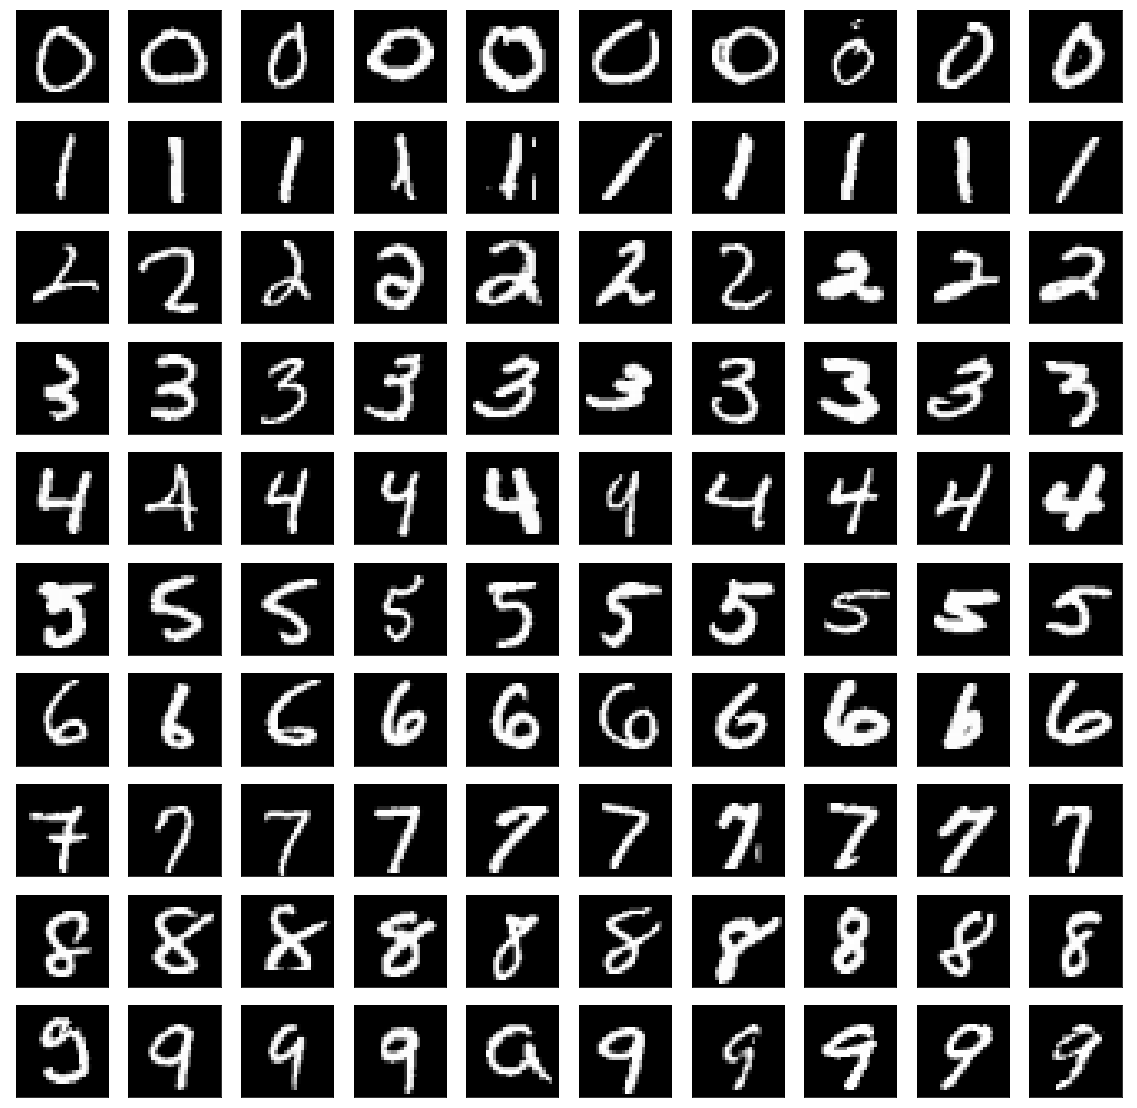
\includegraphics[width=0.5\textwidth]{mnist}
\caption{MNIST Dataset}
\label{fig:mnist_samples}
\end{figure}

State-of-the-art algorithms can classify MNIST with accuracy higher than 0.99, while classical ones, such as SVC or RandomForest, are able to achieve around 0.97\cite{XiaoFashionMNISTNovelImage2017}.


\subsection{Fashion-MNIST}

Xiao et. al.\cite{XiaoFashionMNISTNovelImage2017} propose a novel dataset, called Fashion-MNIST dataset, as a replacement of MNIST dataset for benchmarking machine learning algorithms.  According to \cite{XiaoFashionMNISTNovelImage2017},  Fashion-MNIST brings more challenging to the problem and more representative to modern computer vision tasks. It contains images of fashion products from 10 categories. Fashion-MNIST is comparable to MNIST in every aspects, such as the size of training and testing set, image dimension and data format, hence one can easily  apply existing algorithms that work with MNIST to Fashion-MNIST without any change.

\begin{figure}[h]
\centering
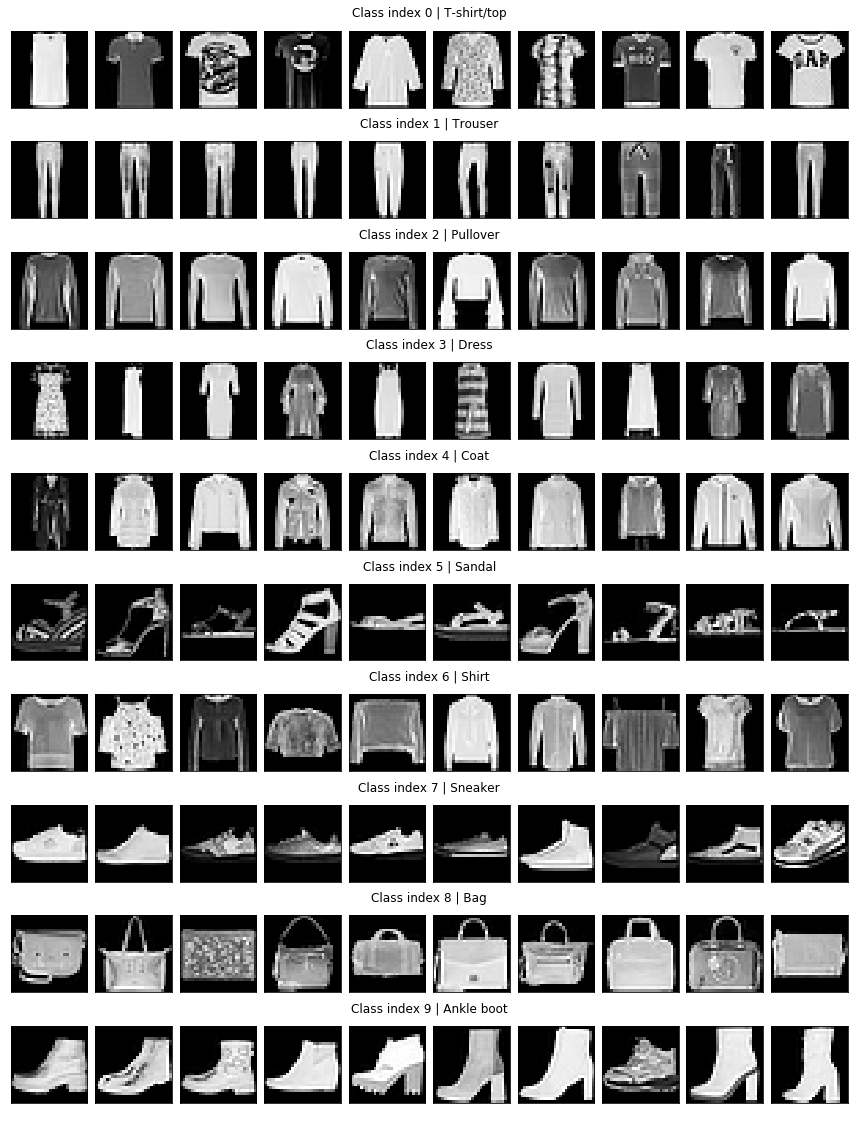
\includegraphics[width=0.6\textwidth]{fashion_mnist}
\caption{Fashion-MNIST Dataset\todo{Figure use same size as MNIST figure}}
\label{fig:fashion_mnist_samples}
\end{figure}

\cite{XiaoFashionMNISTNovelImage2017} also reports benchmarking results of classical machine learning algorithms on Fashion-MNIST. On average, they achieve accuracy between 0.85 to 0.89. According to Fashion-MNIST's page\footnote{https://github.com/zalandoresearch/fashion-mnist}, A. Brock reports the state-of-the-art result  with 0.97 accuracy using Wide Residual Network(WRN)\cite{ZagoruykoWideResidualNetworks2016} and standard data preprocessing and augmentation.


\section{RNN Cell Architectures}
In this section, I will describe architectures or RNN cell evaluated in this thesis.  To make the descriptions concise, I denote notations as follows: 

\begin{itemize}
	\item $\patvector{a}_{t}^{(l)}$ : activation vector of layer $l$ at step $t$
	\item $\patvector{x}_t$ : subset of $x_i \in \patvector{x}$ corresponding to step $t$ and assume to be reshaped into a column vector
\end{itemize}

\subsection{Shallow Cell}
\begin{figure}[!htb]
\centering

\subfloat[Shallow cell\label{fig:s2_network}]{%
       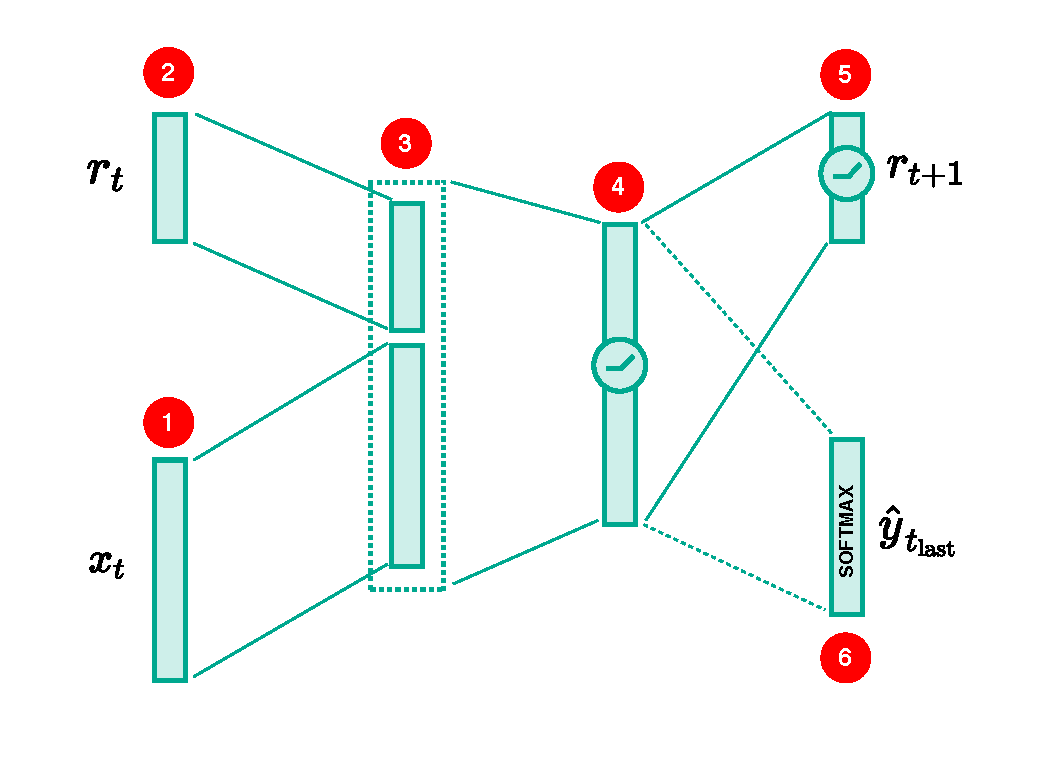
\includegraphics[width=0.48\textwidth]{sketch/s2_network}
     }
     \hfill
     \subfloat[Deep cell\label{fig:s3_network}]{%
       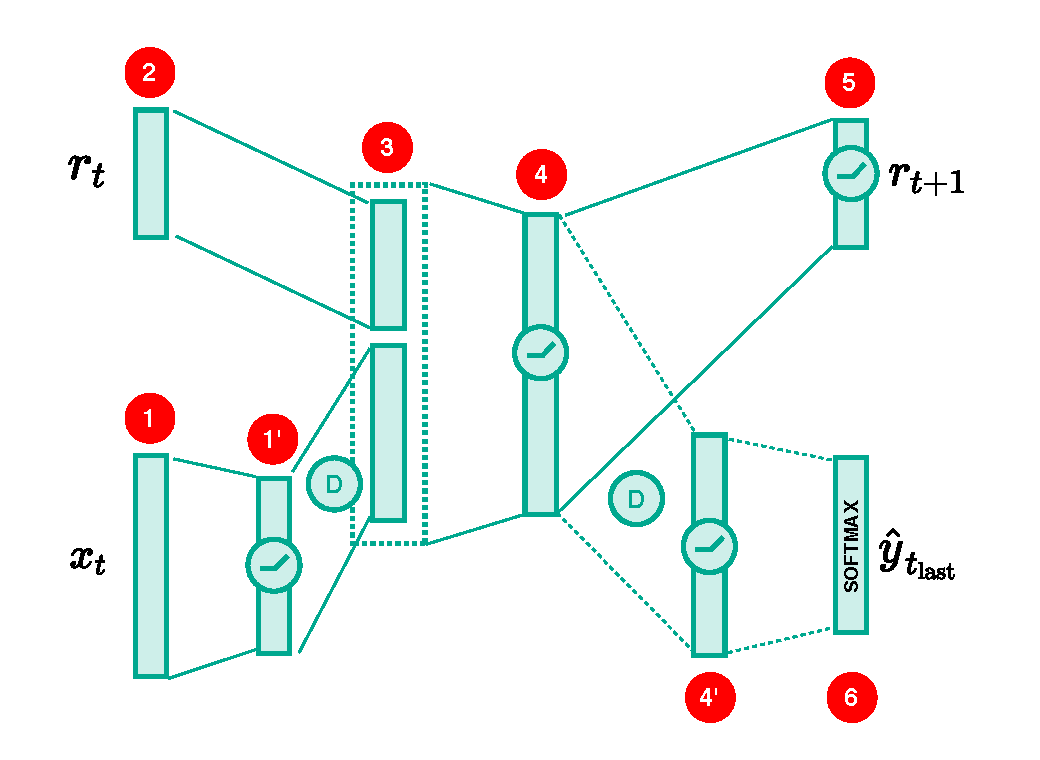
\includegraphics[width=0.48\textwidth]{sketch/s3_network}
     }
\caption{Shallow and Deep Cell Architecture}
\end{figure}

As shown in \addfigure{\ref{fig:s2_network}}, \rnncell{Shallow} cell first concatenates  input $\patvector{x}_t$  \circled{1} and recurrent input $\patvector{r}_t$  \circled{2} at layer \circled{3} as one vector before computing $\patvector{a}_t^{(4)} $ of layer \circled{4}. Then,  the next recurrent input $\patvector{r}_{t+1}$ \circled{5}	 is derived from $\patvector{a}_t^{(4)}$. In the last step $t_{\text{last}}$, the raw output $\patvector{h}$ is computed from $\patvector{a}^{(4)}_{t_{\text{last}}}$ and applied to softmax function to compute class probabilities $\patvector{\hat{y}}$ \circled{6}.



\subsection{Deep Cell Architecture}
%\begin{figure}[!htb]
%\centering
%
%\end{figure}

\addfigure{\ref{fig:s3_network}} illustrates the architecture of  \rnncell{Deep} cell. It can be viewed as  an extension of the Shallow cell with  2 additional layers, namely \circled{1'} and \circled{4'}.  The ideas of introducing the layers are to let \circled{1'} learn representations of the problem, while \circled{4} can focus on combining information from past and current step, which enables \circled{4'} to compute more fine-grained decision probabilities. Dropout is applied at $\patvector{a}^{(1')}_{\cdot}$, and $\patvector{a}^{(4)}_{t_\text{last}}$ for computing $\patvector{a}^{(4')}$.

\begin{figure}[!htb]
\centering

\subfloat[DeepV2\label{fig:deep_4l_network}]{%
       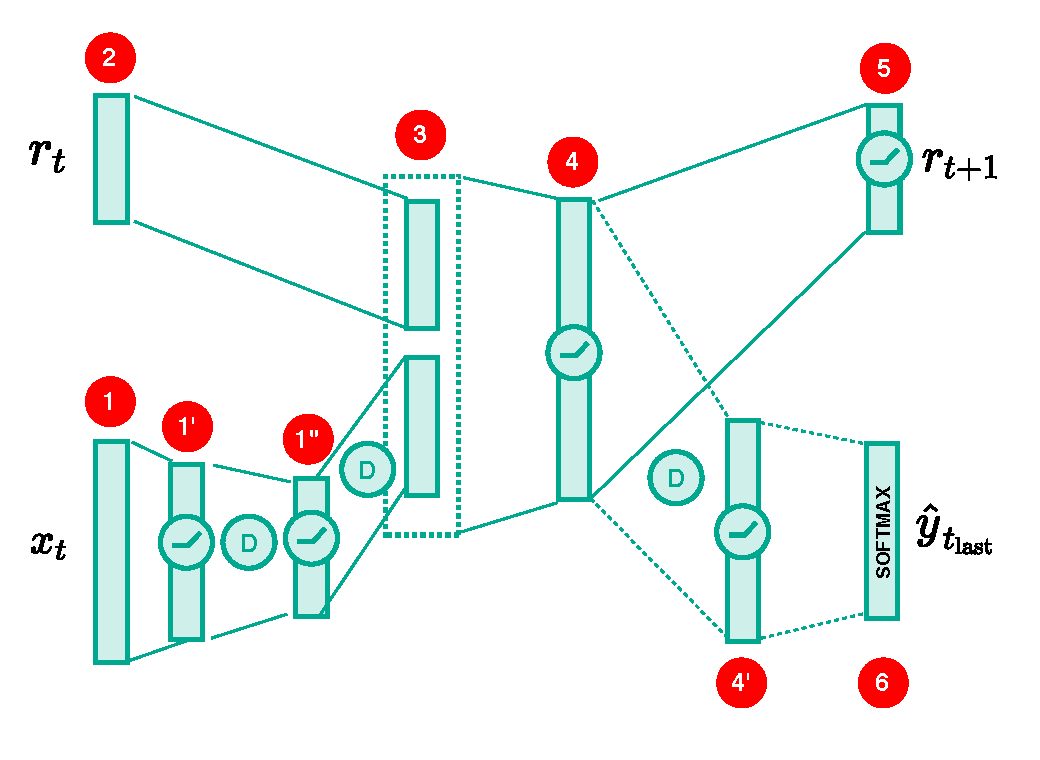
\includegraphics[width=0.48\textwidth]{sketch/deep_4l_network}
     }
     \hfill
     \subfloat[ConvDeep\label{fig:convdeep_4l_network}]{%
       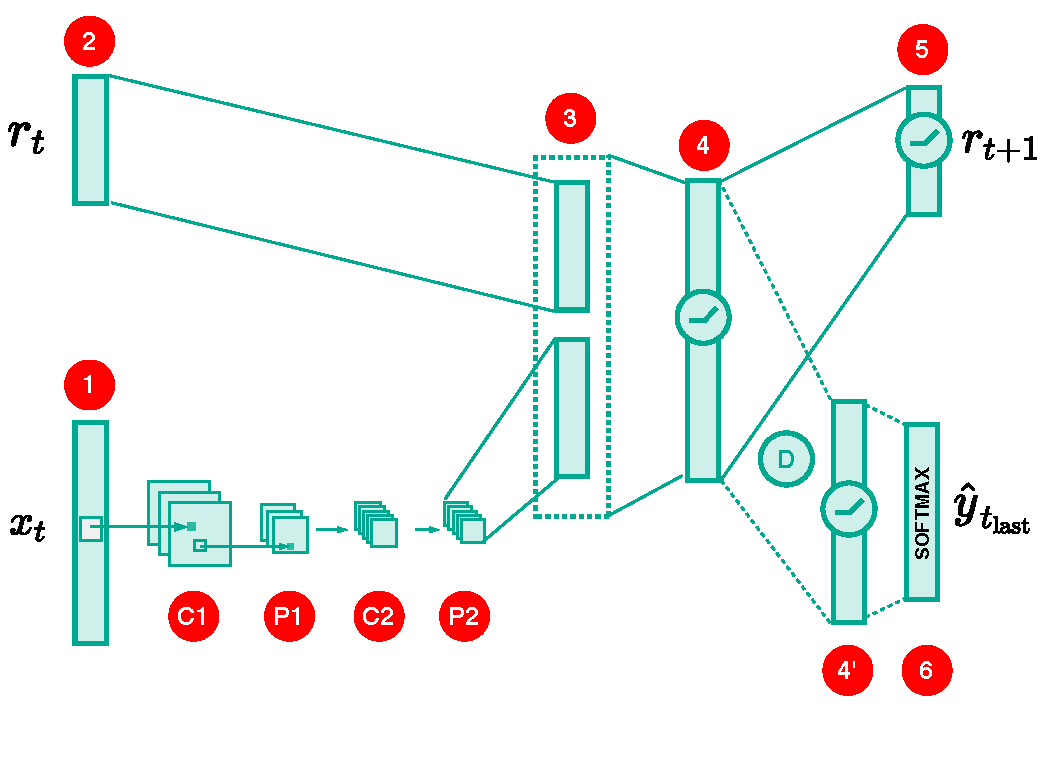
\includegraphics[width=0.48\textwidth]{sketch/convdeep_4l_network}
     }

\caption{DeepV2 and ConvDeep Cell Architecture}
\label{fig:deep_conv_arch}
\end{figure}
%
%
%
%\begin{figure}[!htb]
%\centering
%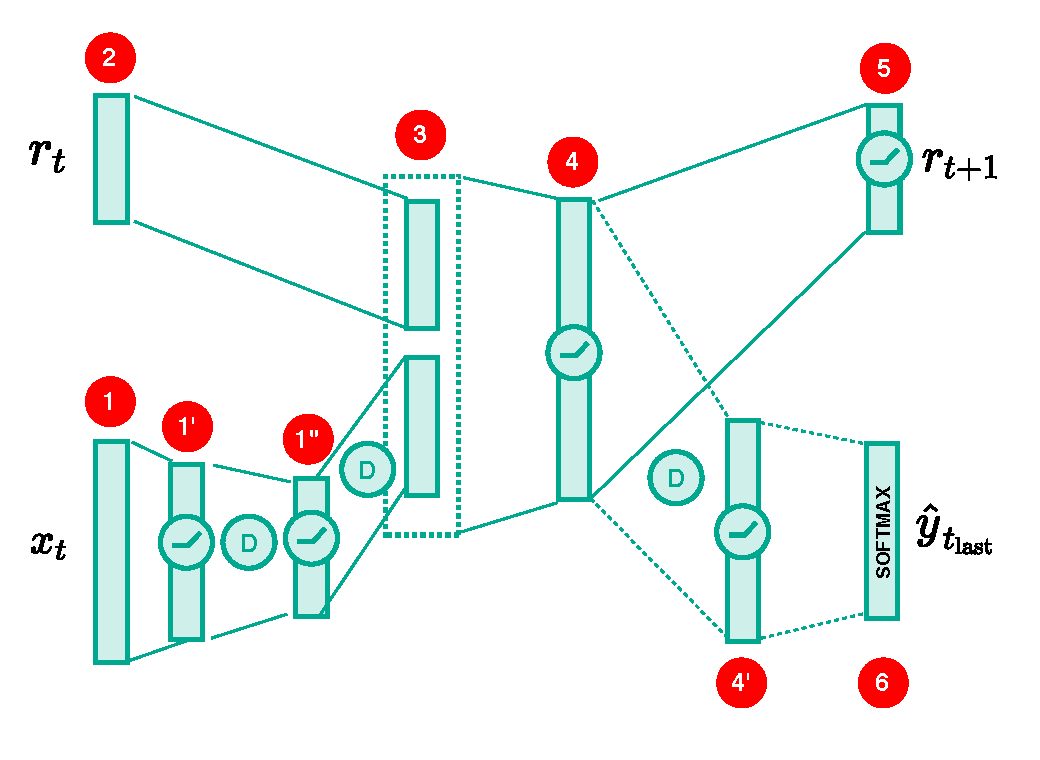
\includegraphics[width=0.6\textwidth]{sketch/deep_4l_network}
%\caption{DeepV2 Cell Architecture}
%\label{fig:deep_4l_network}
%\end{figure}
%
%
%\begin{figure}[!htb]
%\centering
%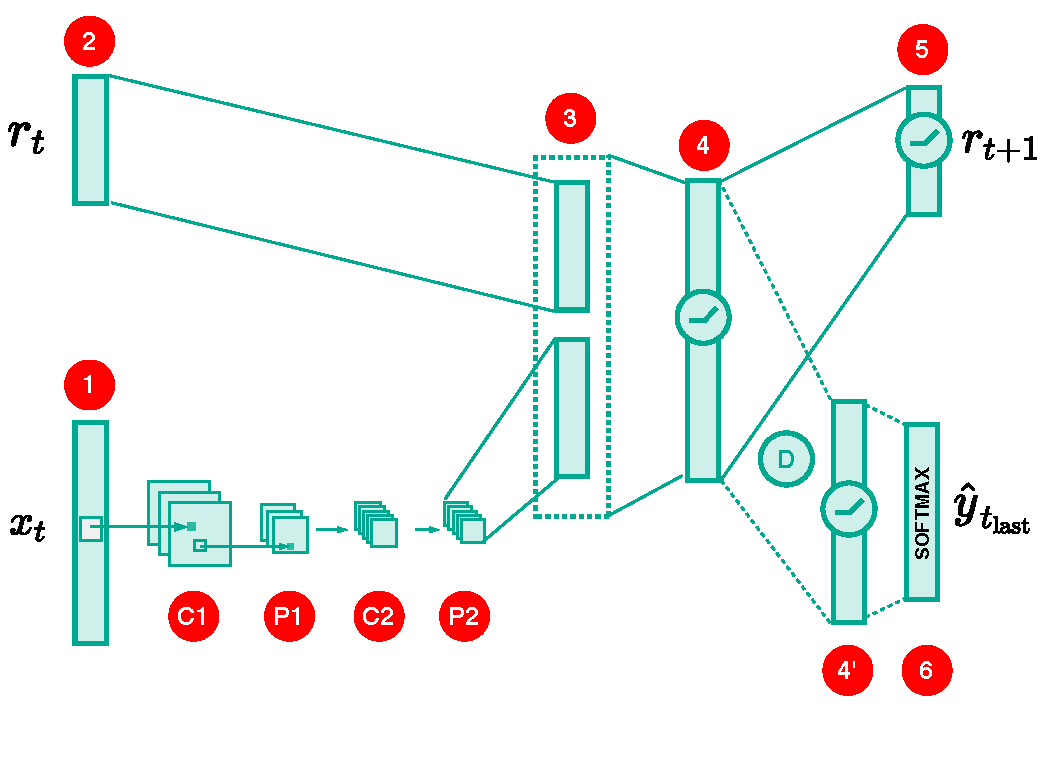
\includegraphics[width=0.6\textwidth]{sketch/convdeep_4l_network}
%\caption{ConvDeep Architecture}
%\label{fig:convdeep_4l_network}
%\end{figure}

Two variations of \rnncell{Deep} cell are also experimented, namely \rnncell{DeepV2} and \rnncell{ConvDeep}, shown on \addfigure{\ref{fig:deep_conv_arch}}. The former has one additional layer \circled{1"} with dropout regularization  between \circled{1'}. On the other hand, the latter replaces fully connected layers between \circled{1} and \circled{3} with 2 convolutional and max pooling layers, \Big[\circled{C1}, \circled{P1}\Big] and \Big[\circled{C2},\circled{P2}\Big].




\section{Setup}\label{sec:setup}
 
 I implemented experiments using TensorFlow\footnote{\url{http://tensorflow.org/}}.  weights $w_{ij} \in \patmatrix{W}$ and biases $b_{j} \in \patvector{b}$ are initialized as follows:
\begin{align*}
	w_{ij} &\sim \Psi( \mu=0, \sigma =0.1, [-2\sigma, 2\sigma]) \\
	b_{j} &= \ln(e^{0.01} - 1)
\end{align*}
where $\Psi(\cdot)$ denotes Truncated Normal Distribution with valid region between $[-2\sigma, 2\sigma]$.

%TODO : Figure normal distribution vs trucated

Activations $\patvector{a}^{(l)}_\cdot$ of layer $l$ is calculated using :
\begin{align*}
	\patvector{h}^{(l)}  &=  	\patmatrix{W}^T \patvector{a}^{(l-1)} - \sigma_{s}(\patvector{b}) \\
	\patvector{a}^{(l)}  &=  	\sigma_{r} (	\patvector{h}^{(l)} )
\end{align*}

where
\begin{align*}
	\sigma_{r} (h_j) &= \max(0, h_j)  \tag{ReLU function}\\
	\sigma_{s} (b_j) &= \log(1+\exp b_j) \tag{Softplus function}
\end{align*}
%TODO : Figure softplus vs relu

The reason of using $\sigma_{s} (b_j)$ for bias term is due to the non positive bias assumption of DTD. Moreover, $\sigma'_{s} (b_j)$ is $(0, \infty)$, as a result the network has more flexibility to adjust decision through back-propagation rather than using $\sigma_{r} (b_j)$. With this setting, the initial value of bias term  $\sigma_{s}(b_j)$ is then 0.01.

Speaking about training methodology, I use Adam\cite{KingmaAdamMethodStochastic2014} optimizer to train networks. Preliminary study shows that relevance heatmaps from networks trained by Adam are less noisy than the ones from other optimizers, such as  Stochastic Gradient Descent(SGD). Number of epochs is set to 200, while dropout probability is 0.5 and batch size is 50.  
Learning rate is not fixed as it is likely that different network architectures requires different value to achieve good performance, hence left adjustable. Table \ref{tab:hyper_summary} summaries the setting of hyperparameters.

%TODO: Figure Heatmaps SGD, RMSProp, Adam
 
 \begin{table}[!htb]
\centering
\begin{tabular}{l|r}
\textbf{Hyperparameter} & \multicolumn{1}{l}{\textbf{Value}} \\ \hline
Optimizer               & Adam                               \\
Epoch     & 200                                \\
Dropout Probability     & 0.5                                \\
Batch size              & 50                                
\end{tabular}
\caption{Hyperparameter Summary}
\label{tab:hyper_summary}
\end{table}
 
Traditionally, number of neurons in each layer ($n^{(l)}$) is  another hyperparameter that we can adjust. However, as the goal is to compare relevance heatmaps from different architectures, those numbers are fixed and chosen in such a way that total number of variables in each architecture are equivalent. \addfigure{\ref{fig:neuron_numbers}} illustrates the details of the settings.

\begin{figure}[!htb]
\centering
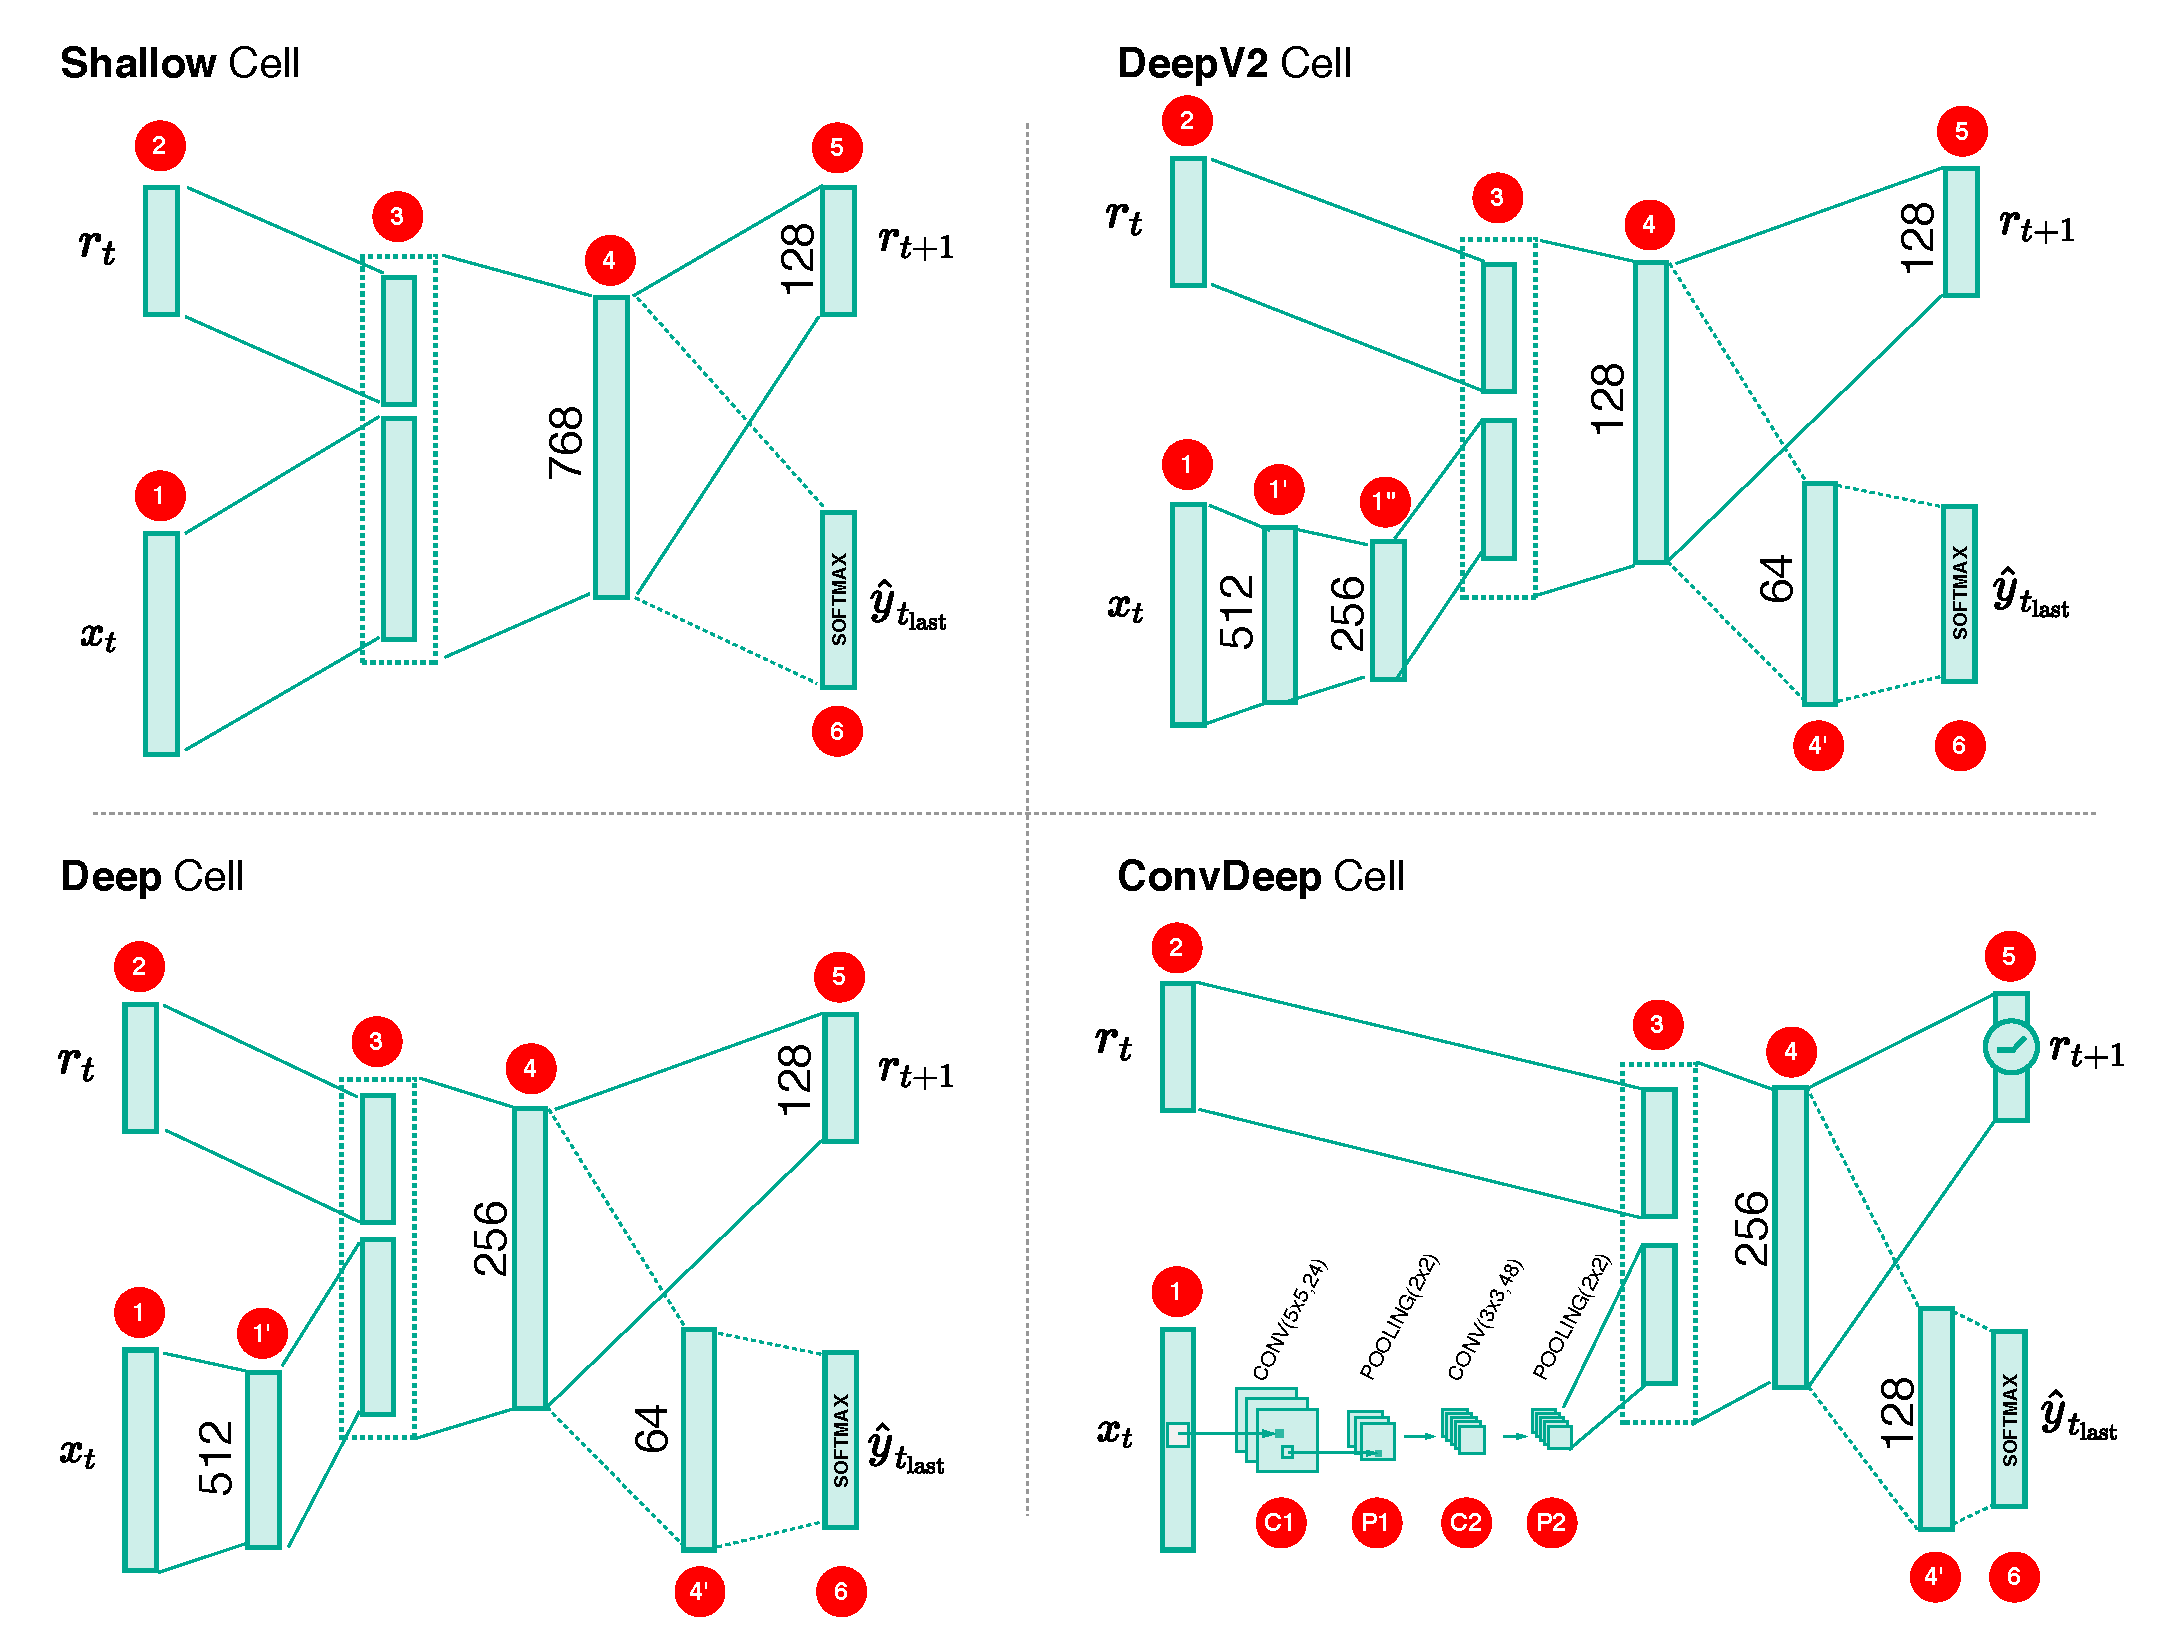
\includegraphics[width=\textwidth]{sketch/neuron_numbers}
\caption{Number of neurons in each layer for each cell architecture}
\label{fig:neuron_numbers}
\end{figure}


\begin{itemize}
	\item \textbf{Shallow Cell} 
$$\{ n^{(4)}\} = \{ 768 \}$$
	\item \textbf{Deep Cell} 
$$\{ n^{(1')}, n^{(4)}, n^{(4')} \} = \{ 512, 256, 64 \}$$
	\item \textbf{DeepV2 Cell} 
$$\{ n^{(1')}, n^{(1")}, n^{(4)}, n^{(4')} \} = \{ 512, 256, 128, 64 \}$$
	\item \textbf{ConvDeep Cell} : 
\begin{align*}
	\{ n^{(C1)}, n^{(P1)} \} &= \{ CONV(5\text{x}5, 24), POOL(2\text{x}2) \} \\
		\{ n^{(C2)}, n^{(P2)} \} &= \{ CONV(3\text{x}3, 48), POOL(2\text{x}2) \} \\
			\{  n^{(4)}, n^{(4')} \} &= \{ 256, 128 \}
\end{align*}
where $CONV(x,y)$ is a convolutional operator with $y$ filters whose kernel size is $\mathbb{R}^{x}$. Similarly, $POOL(x)$ is a pooling operator  with kernel size $\mathbb{R}^{x}$.


\end{itemize}

Noting that, $n^{(5)}$ is set at 128 for all architectures and 0 when the sequence length of the problem is 1. $n^{(6)}$ is equal to the number of categories of a problem, for example $n^{(6)} = 10 $ MNIST. Table \ref{tab:variable_architecture} shows the total numbers of variables in details.

\renewcommand{\arraystretch}{1.2}
\begin{table}[h]
\centering
\begin{tabular}{l|c|c|c|c|}
\cline{2-5}
                                                 & \multicolumn{4}{c|}{\textbf{Sequence Length}} \\ \hline
\multicolumn{1}{|l|}{\textbf{Cell Architecture}} & 1         & 4         & 7         & 14        \\ \hline
\multicolumn{1}{|l|}{\rnncell{Shallow}}                    & 610570    & 355722    & 291210    & 248202    \\ \hline
\multicolumn{1}{|l|}{\rnncell{Deep}}                       & 550346    & 314954    & 271946    & 243274    \\ \hline
\multicolumn{1}{|l|}{\rnncell{DeepV2}}                    & 575050    & 306890    & 263882    & 235210    \\ \hline
\multicolumn{1}{|l|}{\rnncell{ConvDeep}}                   & 647594    & 283178    & 197162    & 197162    \\ \hline
\end{tabular}
\caption{Total variables in each architecture and sequence length}
\label{tab:variable_architecture}
\end{table}


Lastly, as the quality of relevance heatmap depending on performance of the model, the minimum classification accuracy is set as in Table  \ref{tab:min_acc}. 

\begin{table}[h]
\centering
\begin{tabular}{ll}
\multicolumn{1}{l|}{\textbf{Dataset}} & \textbf{Minimum Accuracy} \\ \hline
\multicolumn{1}{l|}{MNIST}            & \multicolumn{1}{r}{0.98}  \\
\multicolumn{1}{l|}{Fashion-MNIST}    & \multicolumn{1}{r}{0.85}  \\
%\multicolumn{1}{l|}{UFI Cropped}                                       &                         \dots
\end{tabular}
\caption{Classification Accuracy Criteria}
\label{tab:min_acc}
\end{table}


\section{Experiment 1 : Sequence Classification}

\subsection{Problem Formulation}
To demonstrate how well RNNs can distribute relevant quantities to input space, I formulated an artificial classification problem in which each image sample $\x$ is column-wise split into non-overlapping $(\x_t)_{t=1}^{T}$.  The RNN classifier needs to summarize information from the sequence $(\x_t)_{t=1}^{T}$ to answer what is the class of $\x$.   

\addfigure{\ref{fig:artificial_problem}} illustrates the setting. Here, a MNIST sample $ \patvector{x} \in \mathbb{R}^{28,28}$ is divided to a sequence of $( \patvector{x}_t \in   \mathbb{R}^{28,7} )_{t=1} ^ 4$. At time step $t$, $\patvector{x}_t$ is presented to the RNN classifier which yields recurrent input $\patvector{r}_{t+1}$ for the next step. For the last step $T$, in this example $T = 4$, the RNN classifier computes $f(\x) \in \mathbb{R}^{10}$ and the class that $\x$ belongs to. 

 \begin{figure}[!hbt]
\centering
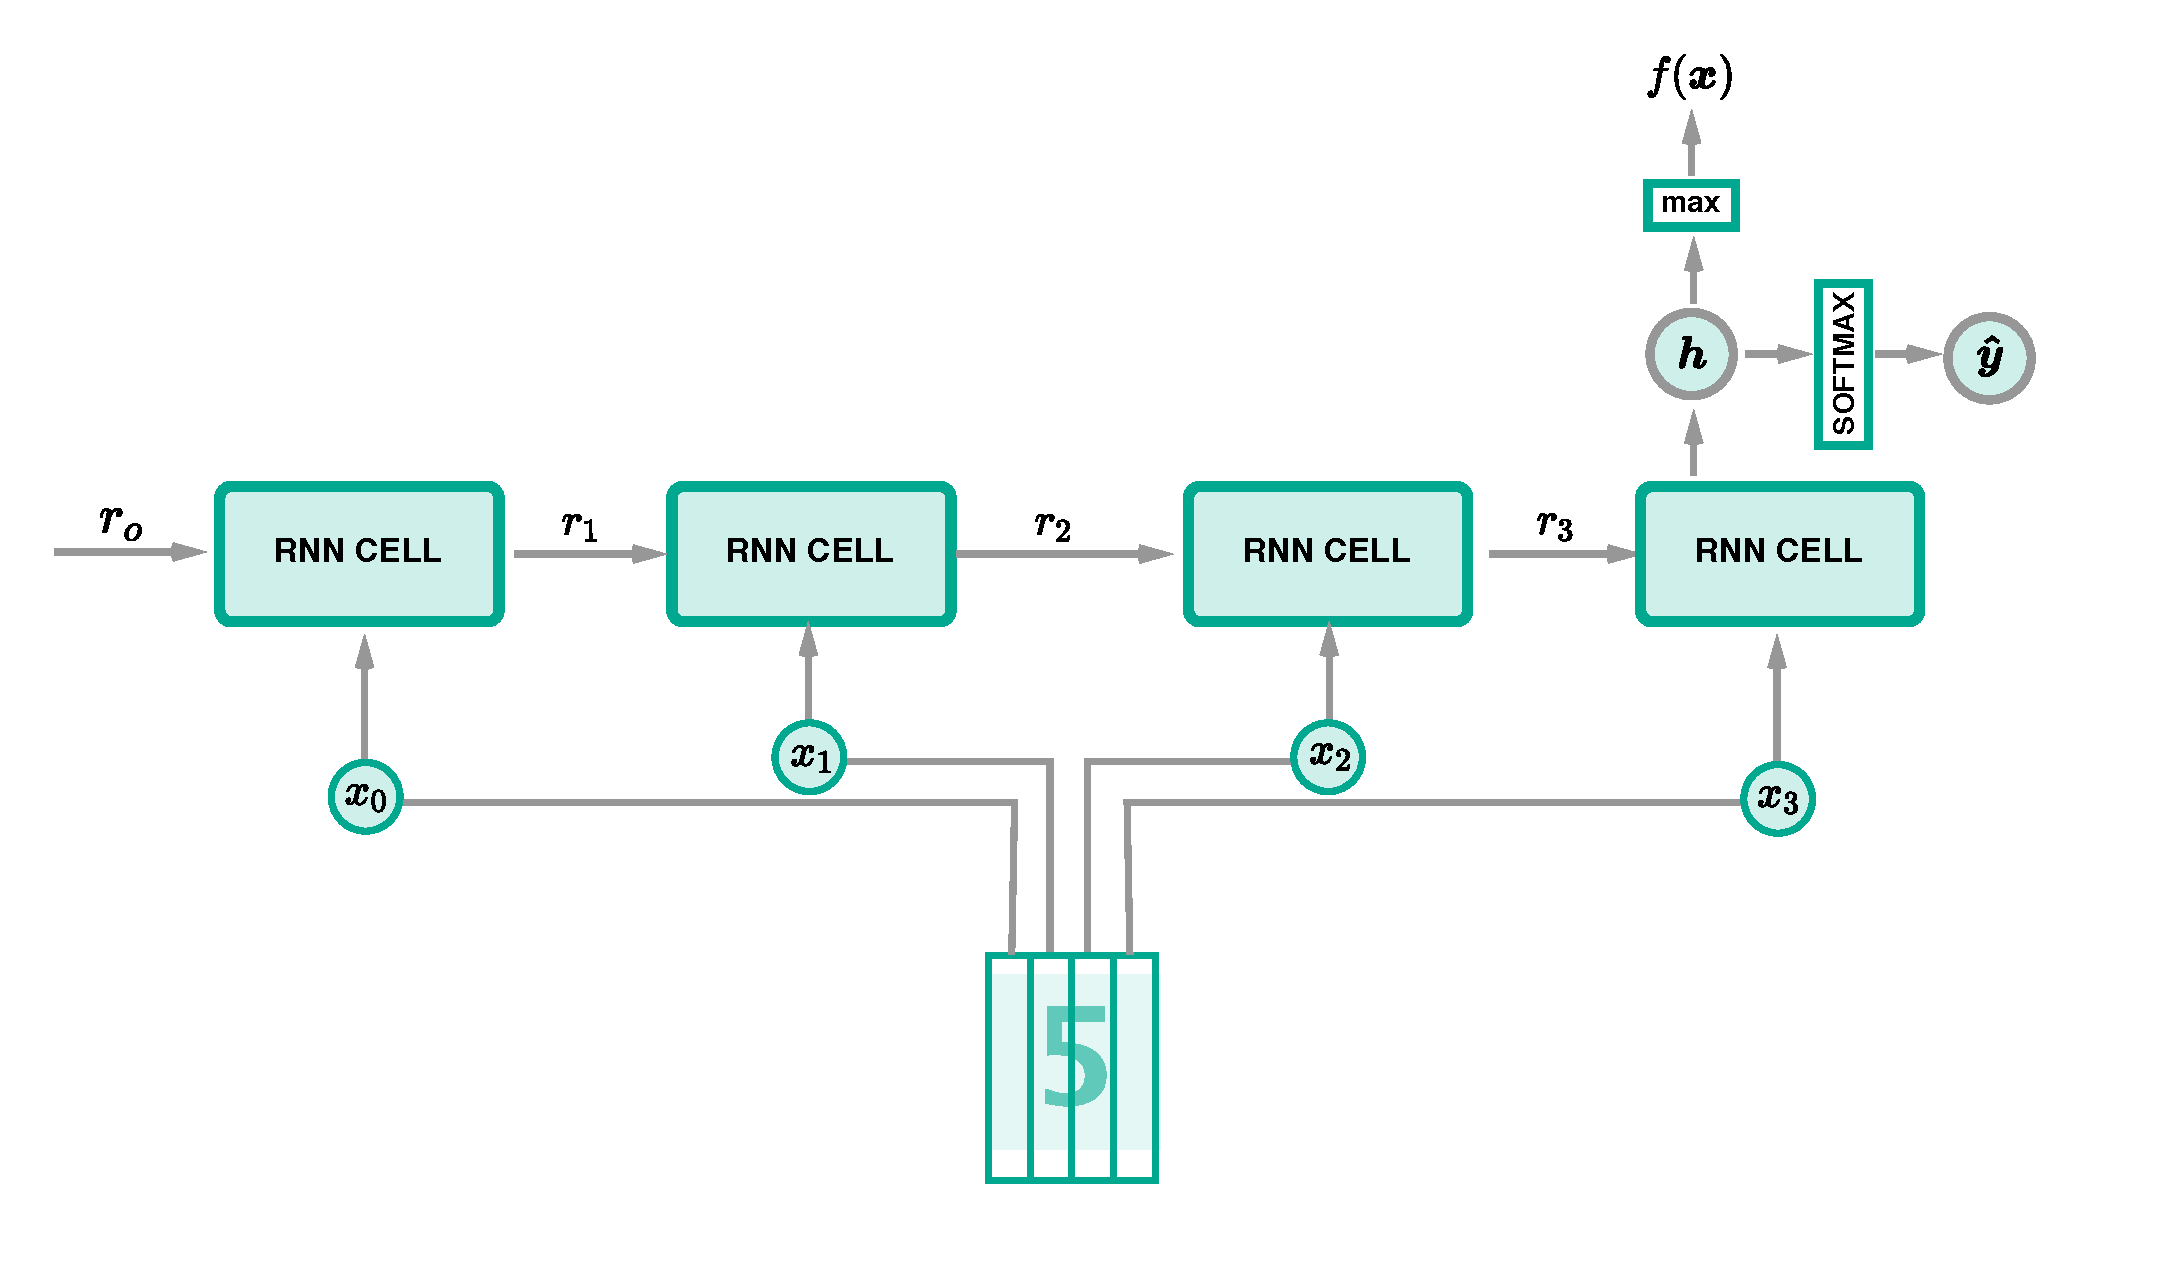
\includegraphics[width=0.9\textwidth]{sketch/artificial_problem}
\caption{General setting of RNN classifiers in this thesis} 
\label{fig:artificial_problem}
\end{figure}

 Denote $g_r$ and $g_{f}$ function that the RNN  with parameters $\boldsymbol{\theta}$ uses to compute $\patvector{r}_{t+1}$ and $f(\x)$ respectively. The overall computation can be summarized as follows: 
 \begin{align*}
 	\patvector{r}_{t+1} &= g_r(\patvector{\theta}, \patvector{x_t}, \patvector{r_t}) \\
 	 &\ \ \vdots\\
f(\x) &= g_{h}(\patvector{\theta}, \patvector{x}_{t_{\text{last}}},  \patvector{r}_{t_{\text{last}}}) \\
 	\patvector{\hat{y}} &= \text{softmax}(f(\x)),
 \end{align*}
 where $\patvector{\hat{y}}$ is the class probabilities and $\patvector{r}_0 = \patvector{0}$.   To explain the model,  $R(\x)$ is set to the value of $f(\x)$ that is corresponding to the true target class.
 
 \todo{Figure figure show how R(x) is set?}
 
 
\renewcommand{\arraystretch}{1.5}
\begin{table}[h]
\centering
\begin{tabular}{l|l|l|l|l|}
\cline{2-4}
                                            & \multicolumn{3}{c|}{Sequence Length}                                                               \\ \hline
\multicolumn{1}{|c|}{Dataset}               & \multicolumn{1}{c|}{1} & \multicolumn{1}{c|}{4} & \multicolumn{1}{c|}{7}  \\ \hline
\multicolumn{1}{|l|}{MNIST / FashionMNIST} &        $ \mathbb{R}^{28,28}  $              &          $ \mathbb{R}^{28,7}  $               &         $ \mathbb{R}^{28,4}  $                            \\ \hline
%\multicolumn{1}{|l|}{UFI-Cropped}           &                        &                        &                        &                         \\ \hline
%\multicolumn{1}{|l|}{}                      &                        &                        &                        &                         \\ \hline
\end{tabular}
\caption{Dimensions of $\patvector{x}_t$ for each dataset and sequence length}
\label{tab:seq-length}

\end{table}
\renewcommand{\arraystretch}{1}

%In this section, I am going to present what I have  found from experiments. First, I am going to discuss results from MNIST and then move on to ones from Fashion-MNIST. Moreover, I will use \rnncellseq{CELL\_NAME}{SEQ} convention to denote a RNN network with CELL\_NAME cell trained on a sequence length SEQ. For example, \rnncellseq{Deep}{7} means a RNN with Deep cell architecture trained on data whose $\patvector{x}^{(\alpha)}$ is a sequence of length 7.


\subsection{Result}
I began this preliminary experiment  with Shallow and Deep architecture. They were trained on MNIST and FashionMNIST with sequence length $T = \{1, 4, 7\}$. Table \ref{tab:seq-length} shows dimensions of $\patvector{x}_t$ for different sequence length and Table \ref{tab:mnist_model_acc} summaries accuracy of the trained models. To simplify the manuscript, I am going to use \textit{\rnncellseq{ARCHITECTURE}{T}} convention to denote a RNN with \textit{ARCHITECTURE} trained on sequence length \textit{T}. For example, \rnncellseq{Deep}{7} refers to the Deep RNN architecture trained on $(\x_t \in \mathbb{R}^{28,4} )_{t=1}^{7}$.


\begin{table}[]
\centering
\begin{tabular}{lrr}
\textbf{}                  & \multicolumn{1}{c}{\textbf{Shallow}} & \multicolumn{1}{c}{\textbf{Deep}} \\ \hline
\multicolumn{1}{l|}{SEQ-1} & xx.xx\%                              & xx.xx\%                           \\
\multicolumn{1}{l|}{SEQ-4} & xx.xx\%                              & xx.xx\%                            \\
\multicolumn{1}{l|}{SEQ-7} & xx.xx\%                              & xx.xx\%
\end{tabular}
\caption{Model Accuracy}
\label{tab:mnist_model_acc}
\end{table}


 \begin{figure}[h]
\centering
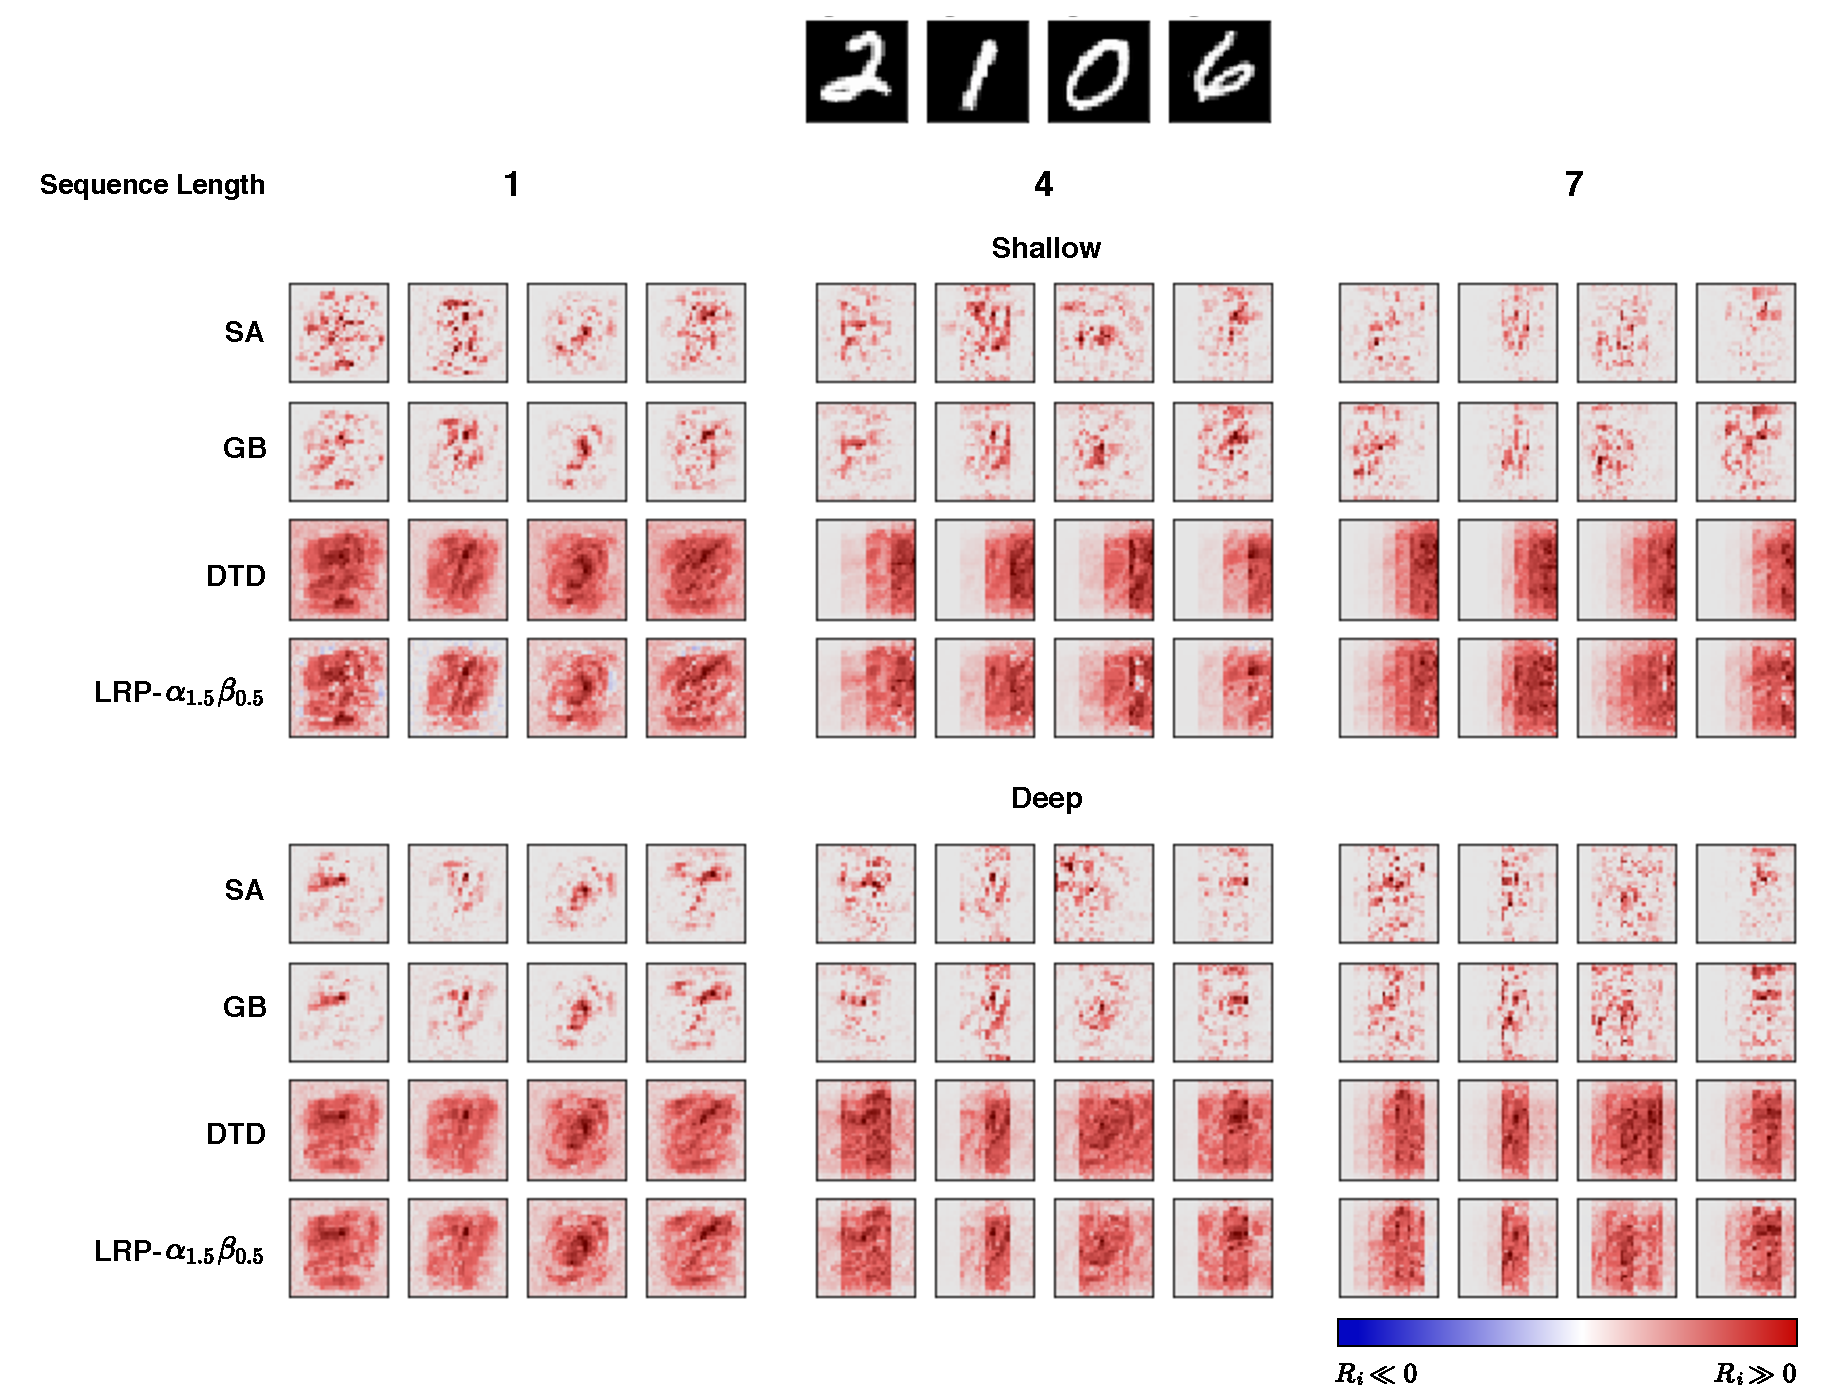
\includegraphics[width=0.8\textwidth]{sketch/mnist_experiment}
\caption{Relevance heatmaps from Shallow and Deep Cell trained on MNIST with different sequence lengths}
\label{fig:mnist_experiment}
\end{figure}


\addfigure{\ref{fig:mnist_experiment}} shows relevance heatmaps from Shallow and Deep architecture trained on MNIST.  We can see general characteristics of each explanation technique. In particular, sensitivity analysis(SA) and guided backprop(GB) heatmaps are sparse, while the ones from deep Taylor decomposition(DTD) are more diffuse throughout $\x$.  When applying these techniques to \rnncellseq{Shallow}{1}  and \rnncellseq{Deep}{1}, the relevance heatmaps look similar regardless of the architectures.  As the sequence length is increased, SA and GB heatmaps are still almost identical  for \rnncellseq{Shallow}{4,7} and \rnncellseq{Deep}{4,7}. However, this is not the case for DTD.  From the figure, we can see that \rnncellseq{Shallow}{4,7} and  \rnncellseq{Deep}{4,7} return significantly different relevance heatmaps from DTD method.  In particular,  \rnncellseq{Shallow}{4,7} 's heatmaps are mainly concentrated on the right part of $\x$ associating to last time steps, while  \rnncellseq{Deep}{4,7}'s ones are appropriately highlighted at the actual content area of $\x$.


 \begin{figure}[h]
\centering
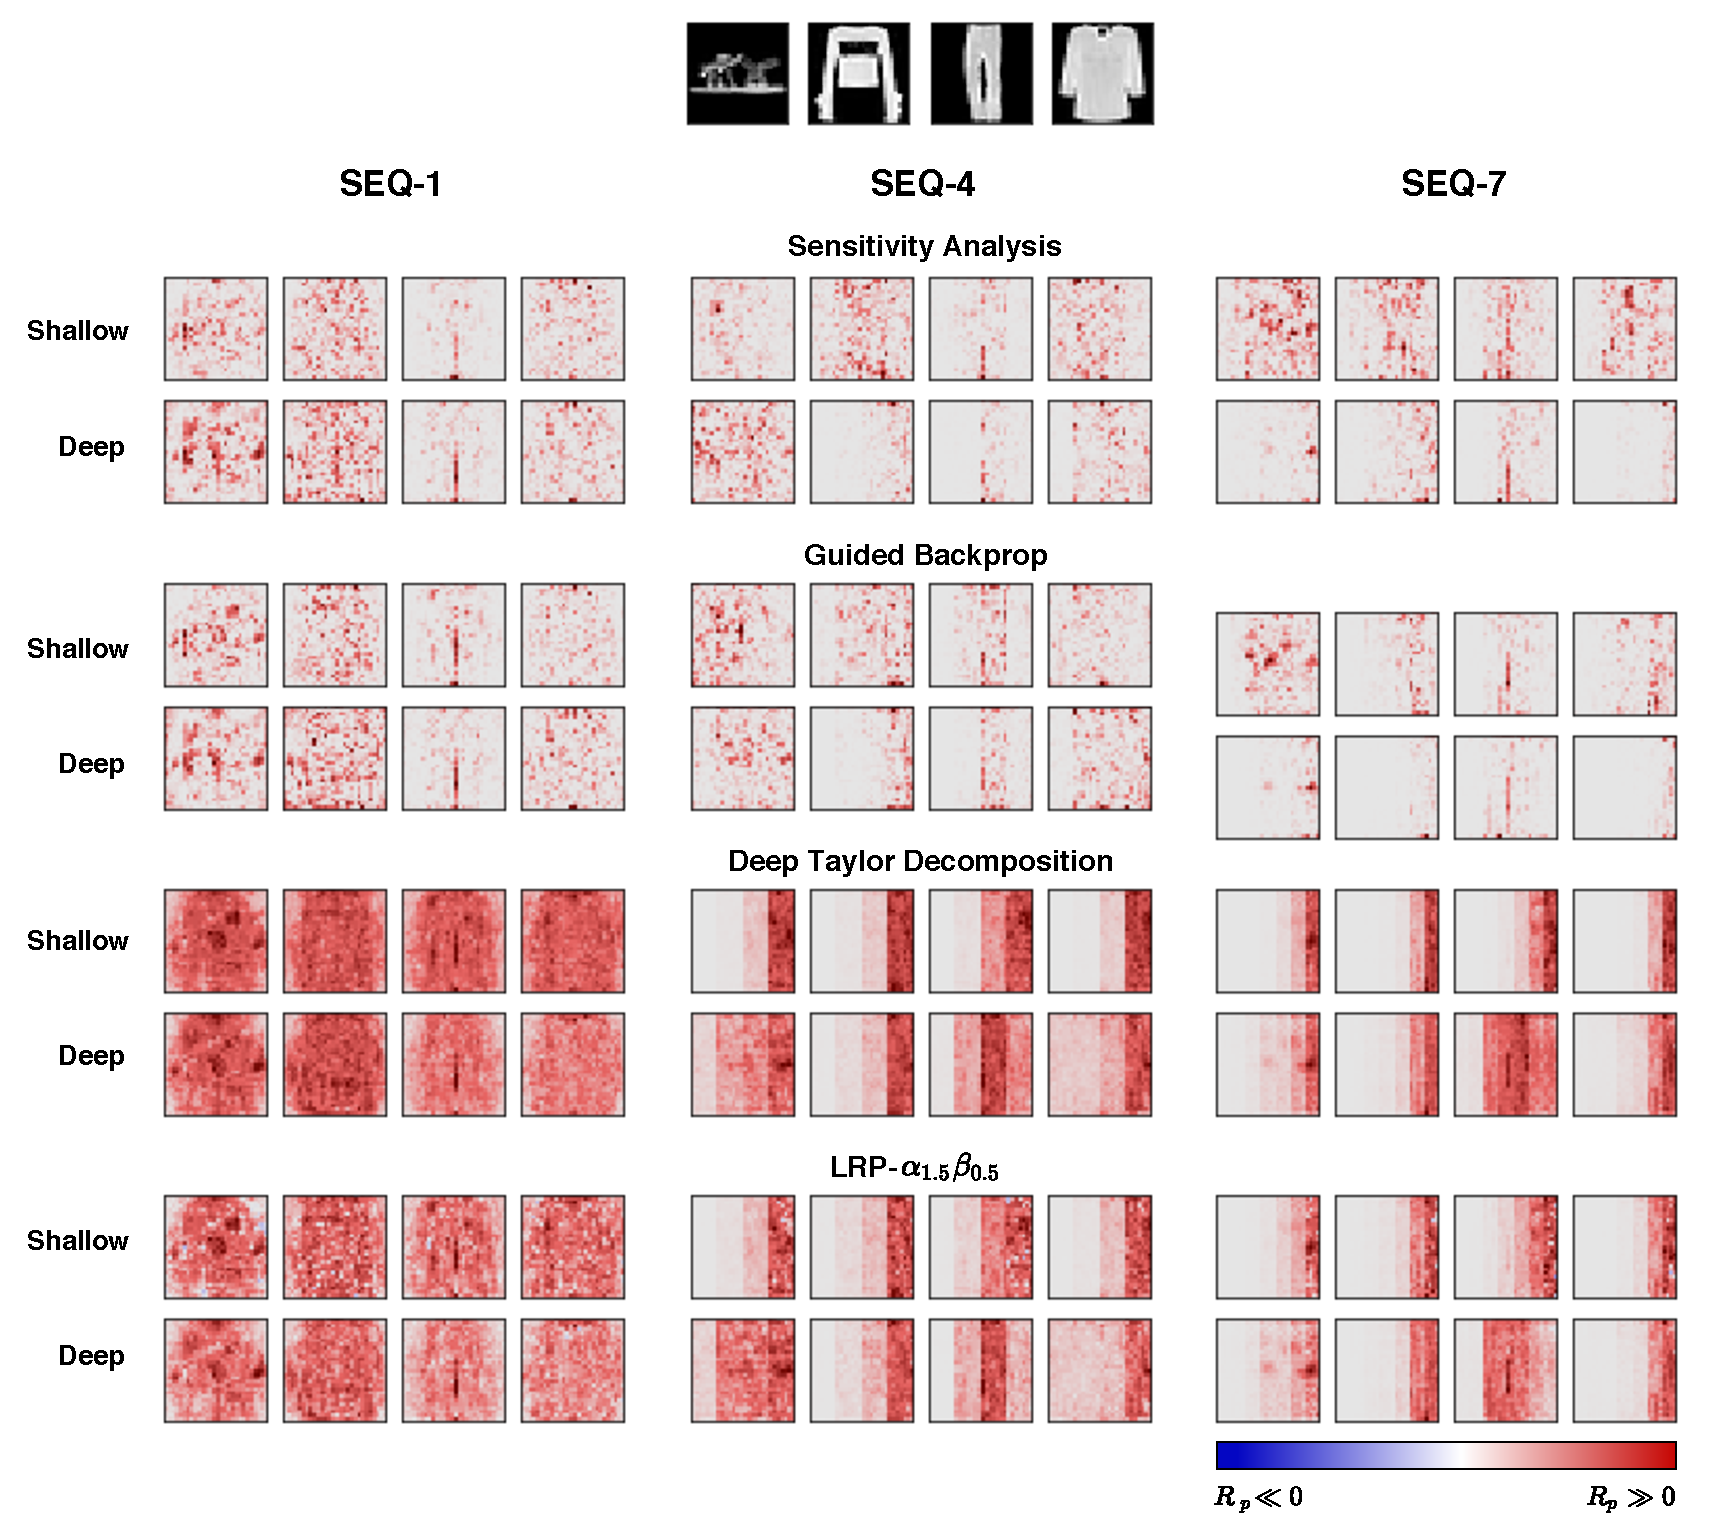
\includegraphics[width=0.8\textwidth]{sketch/fashion_mnist_experiment}
\caption{Relevance heatmaps from Shallow and Deep Cell trained on FashionMNIST with different sequence lengths}
\label{fig:fashion_mnist_experiment}
\end{figure}

Relevance heatmaps of Shallow and Deep architecture trained on  FashionMNIST  are shown on \addfigure{\ref{fig:fashion_mnist_experiment}}. Similar to MNIST, we do not see any remarkable difference on SA and GB heatmaps of the two architectures : only that \rnncellseq{Deep}{4,7} produces slightly more sparse heatmaps. Although the wrong concentration issue of DTD  seems to appear on both \rnncellseq{Shallow}{4,7}'s and \rnncellseq{Deep}{4,7}'s heatmaps, we still can observe proper highlight from Deep architecture on some samples. For example, the trouser sample, we can see  that \rnncellseq{Deep}{4,7} architecture manage to distribute high relevance scores to area of the trouser. Latent features of FashionMNIST  might be one of the reasons why Deep architecture does not distribute relevance scores to early steps for the FashionMNIST samples. Consider \textit{Shoe} and \textit{Ankle Boot} samples in \addfigure{\ref{fig:fashion_mnist_samples}}. One can see that  their front part are similar and only the heel part that determines the differences between the two categories.




 \begin{figure}[ht!]
\centering
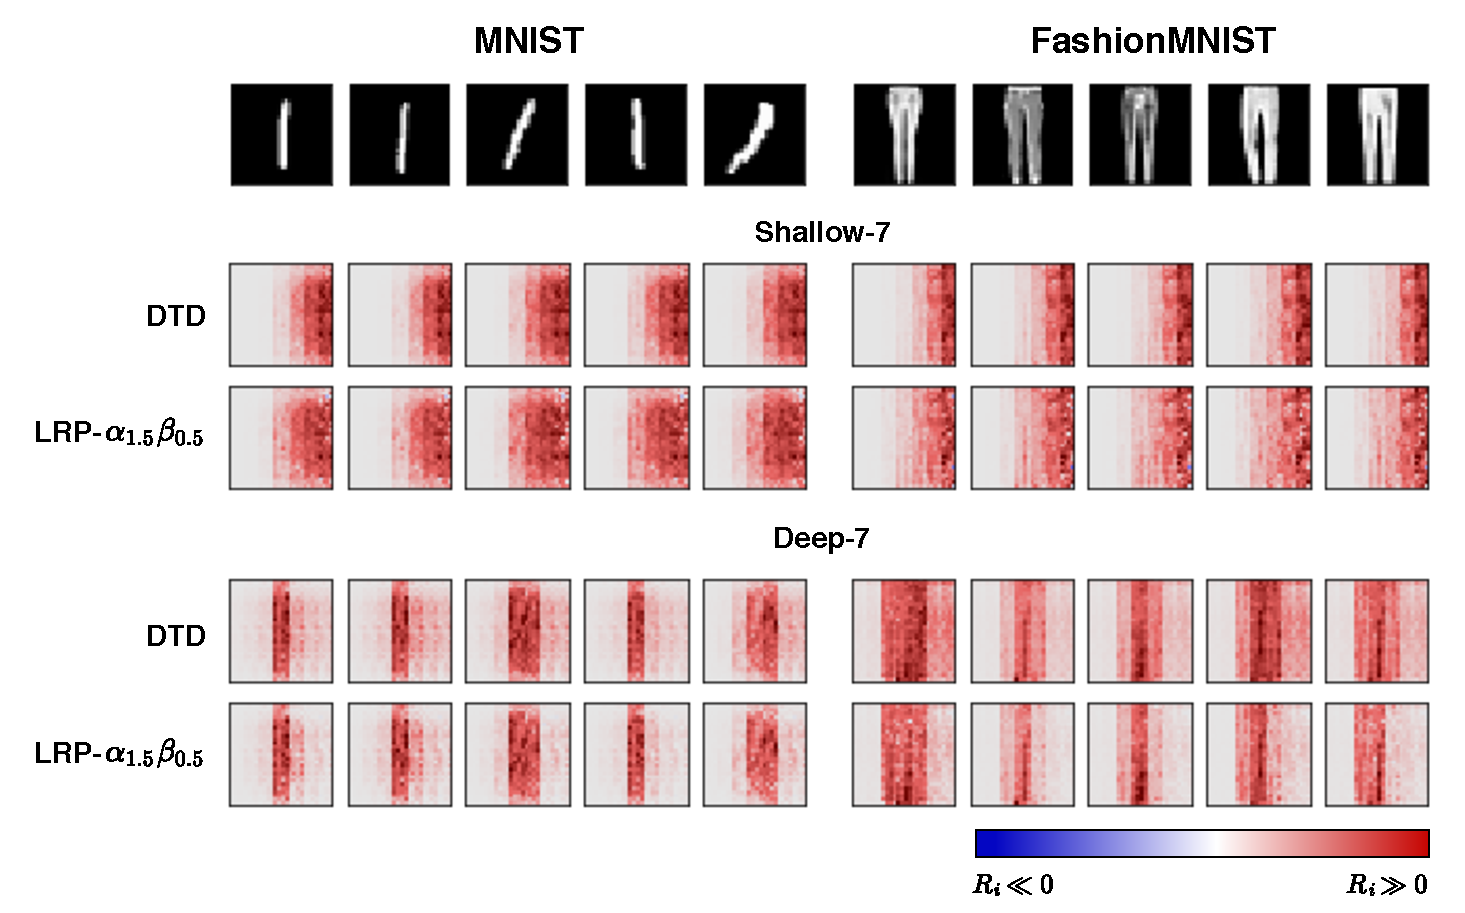
\includegraphics[width=\textwidth]{sketch/class_1_comparison}
\caption{DTD relevance heatmaps of MNIST \textit{Class 1} and FashionMNIST \textit{Class Trouser} samples from \rnncellseq{Shallow}{7} and \rnncellseq{Deep}{7}. }
\label{fig:class_1_comparison}
\end{figure}

\addfigure{\ref{fig:class_1_comparison}} presents relevance heatmaps of MNIST \textit{Class 1} and FashionMNIST \textit{Class Trouser} samples. These samples were chosen to emphasize the impact of RNN architecture on DTD explanation. In particular,  these samples have $\x_{t'}$ containing features  primarily locating at the center, or middle of the sequence, hence appropriate relevance heatmaps should be highlighted at $\x_{t'}$ and possibly its neighbors.  As expected, we can see \rnncellseq{Deep}{7} produces sound results in which the  heatmaps have high intensity value where $\x_{t'}$ approximately locate, while \rnncellseq{Shallow}{7} mainly assigns relevance quantities to $\x_{t}$ for $t \approx T$. \addfigure{\ref{fig:exp1_dist_plot}} further shows a quantitive evidence of this problem. Here, distribution of relevance score from \rnncellseq{Shallow}{7} and \rnncellseq{Deep}{7} are plotted across time step $t = \{ 1, \dots, 7 \}$. The distributions are computed from all test samples in MNIST \textit{Class 1} and FashionMNIST \textit{Class Trouser} respectively as well as the data distributions that are derived from pixel intensity values.  We can see that \rnncellseq{Deep}{7}'s relevance distributions are similar to the data distributions, while  \rnncellseq{Shallow}{7}'s ones diverge completely. Particularly,  one can see that \rnncellseq{Shallow}{7} distributes more than 90\% of relevance scores to the last 3 steps, namely $\x_5$, $\x_6$ and $\x_7$.


 \begin{figure}[h]
\centering
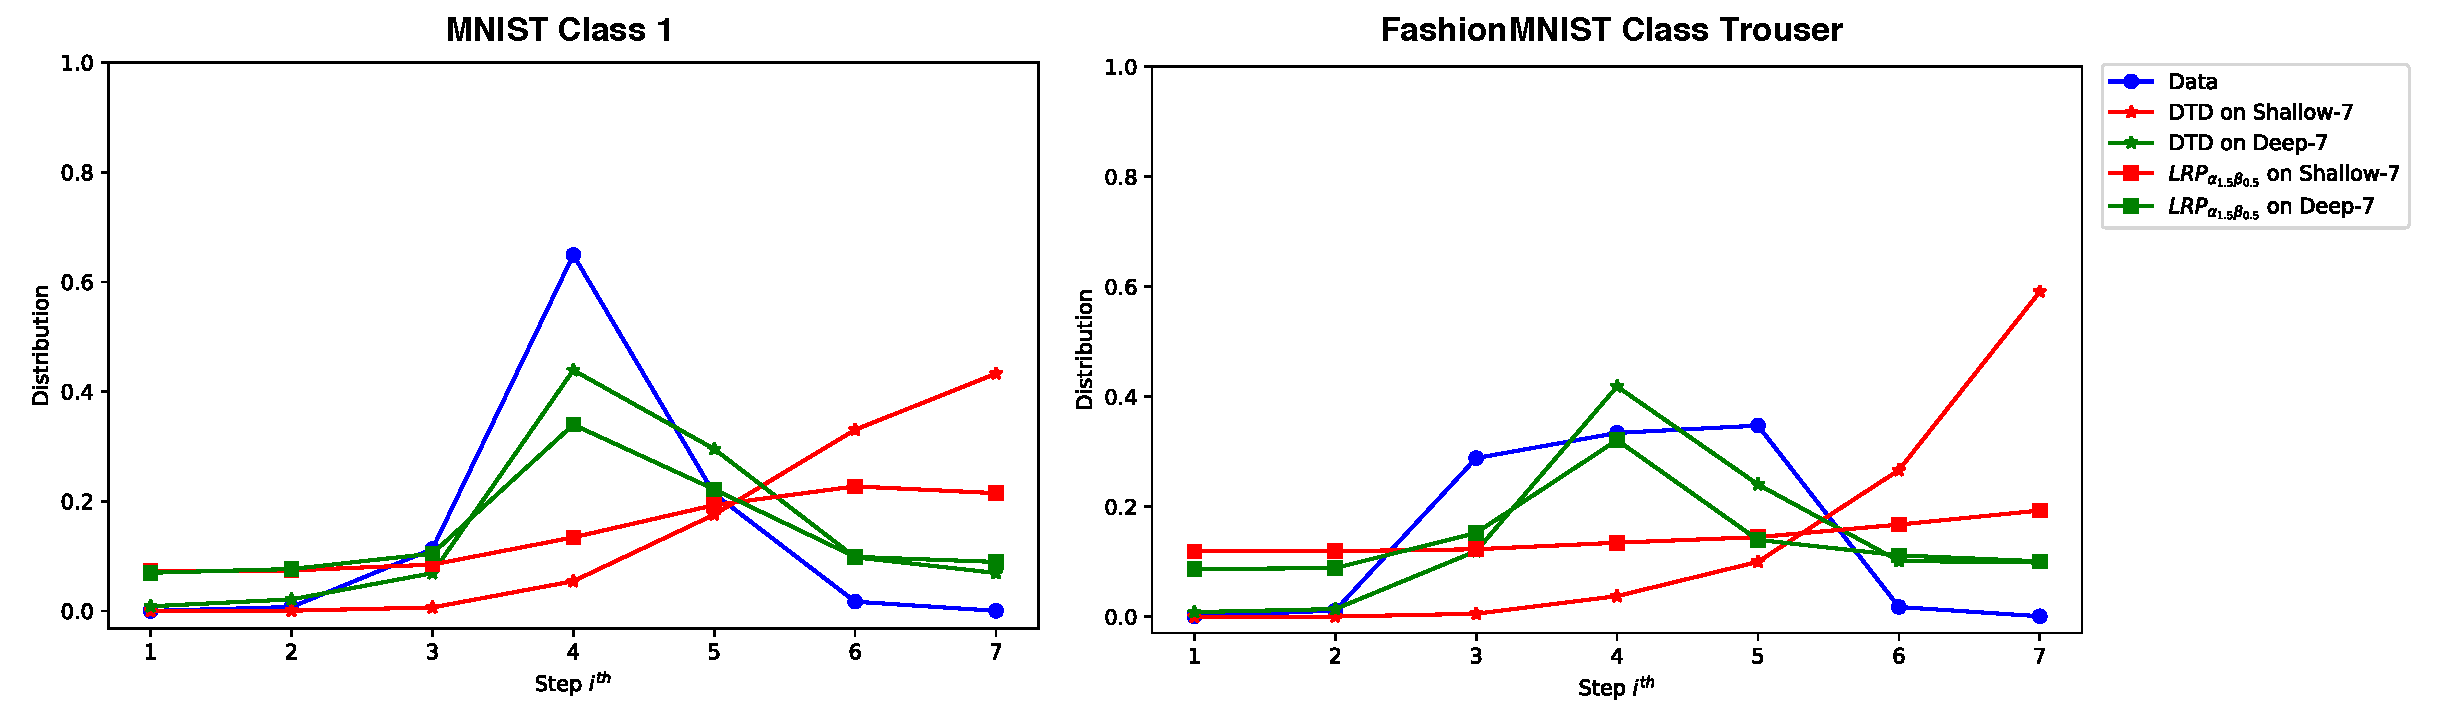
\includegraphics[width=\textwidth]{sketch/exp1_dist_plot}
\caption{Pixel intensity and DTD relevance distribution from \rnncellseq{Shallow}{7} and \rnncellseq{Deep}{7} averaged over MNIST \textit{Class 1} and FashionMNIST \textit{Class Trouser} test population.} 
\label{fig:exp1_dist_plot}
\end{figure}

\subsection{Summary}
Results from this first experiment seem to suggest that choice of RNN architectures has an impact on quality of its explanation.  In particular,  as presented in \addfigure{\ref{fig:class_1_comparison}} and \addfigure{\ref{fig:exp1_dist_plot}}, quality of deep Taylor decomposition(DTD) explanation is significantly influenced by the architecture. In contrast, we do see such notable effect from sensitivity analysis(SA) and guided backprop(GB) method.  In the following experiment, I am going to present a methodical evaluation of this impact in detail.



\section{Experiment 2 : Majority Sample Classification} \label{sec:exp2}
   
 \begin{figure}[h]
\centering
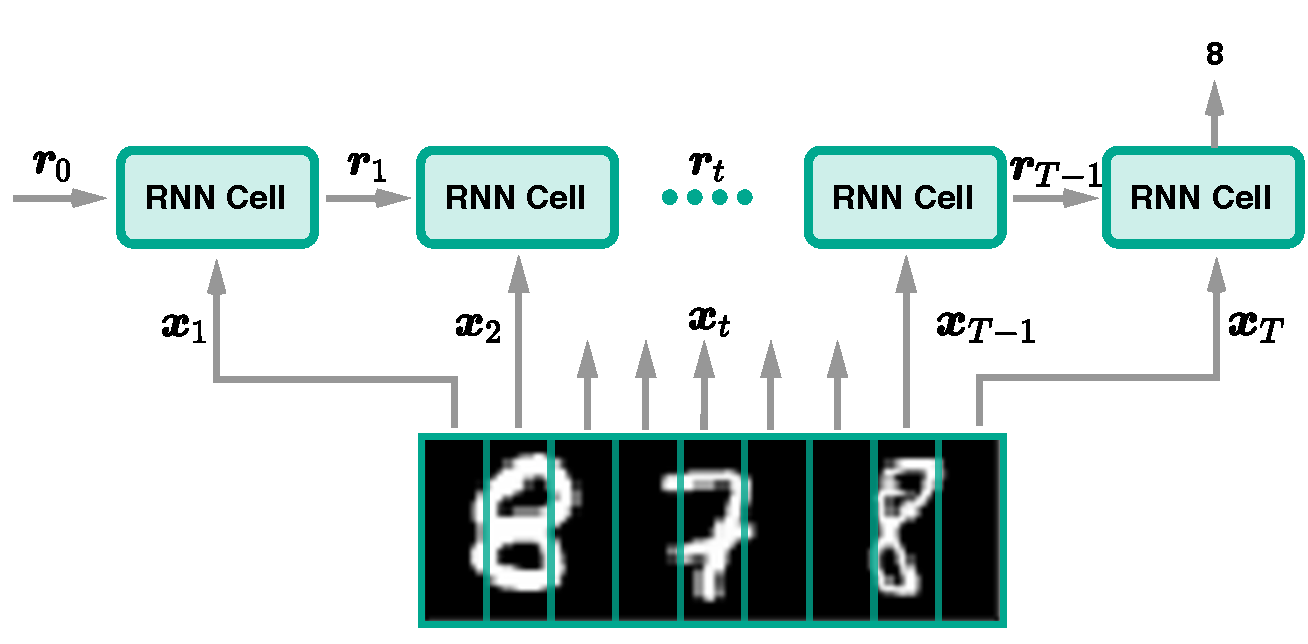
\includegraphics[width=0.7\textwidth]{sketch/artificial_problem_3digits}
\caption{Majority Sample Classification Problem} 
\label{fig:artificial_problem_3digits}
\end{figure}

\subsection{Problem Formulation} \label{sec:exp2_prob_formulate}
When neural network are trained, one can apply explantation techniques to the models to get relevance heatmaps of samples.  The heatmap of sample $\x$ illustrates important features in $x$ that the trained network utilizes to perform its objective prediction,  such as classification.  Therefore, one needs to know the ground truth of these latent features in order to methodologically evaluate how well the model distributes  relevance scores to $\x$'s input space. However,  this knowledge is not trivial to find as it is an incident from the optimization process in high-dimensional space that we in fact seek to understand.

To alleviate this challenge, I constructed two artificial datasets using samples from  MNIST and FashionMNIST respectively. Let's consider MNIST. The new dataset was constructed as follows: each original sample $\widetilde{\x} \in \mathbb{R}^{28,28}$, I randomly selected 2 additional samples : one from the same class of $\widetilde{\x}$ and the other one from a different class. Then, these 3 samples are concatenated in random order yielding a sample $\x \in \mathbb{R}^{28,84}$ of the new dataset. 

With this construction procedure, one possible objective  is to train RNNs to predict the majority class in each sequence $(\x_t )_{t=1}^{T}$. For example, consider $\x = \{ 8, 7, 8\}$ shown in \addfigure{\ref{fig:artificial_problem_3digits}}, the majority class here is \textit{Class 8}. Because we already know time step $t'$ that are corresponding to original samples $\widetilde{\x}$ belonging to the majority group in each sequence $\x$, we can simply compute percentage of relevance scores assigned to $t'$ to quantitively  evaluate explainability  of a RNN architecture. 

I also introduces two additional variation of Deep architecture, namely DeepV2 and ConvDeep. DeepV2 has one more layer after the first fully-connected layer, while ConvDeep instead employs a sequence of convolutional and pooling operation after the input layer. Figure X shows details of the architectures. 



 %Table x show accuracy sf

\subsection{Result}


\begin{table}[h]
\begin{center}
\begin{tabular}{l c|c|c|}
\cline{3-4}
& &
\multicolumn{2}{c|}{\parbox{3.5cm}{ \vskip 1mm \centering \textbf{Accuracy} \vskip 1mm}} \\ \hline
\multicolumn{1}{|l|}{\textbf{Cell Architecture}} & \textbf{No. variables} & \textbf{MNIST} & \textbf{FashionMNIST} \\ \hline
\multicolumn{1}{|l|}{Shallow}    & 184330                 & 98.39\% & 90.15\% \\ 
\multicolumn{1}{|l|}{Deep}       & 153578                 & 98.42\% & 90.60\% \\ 
 \multicolumn{1}{|l|}{DeepV2}     & 161386                 & 98.38\% & 90.43\% \\
\multicolumn{1}{|l|}{ConvDeep}   & 151802                 & 99.07\% & 92.43\%  \\ \hline 
\end{tabular}

\end{center}
\caption{Number of trainable variables and model accuracy for Majority Sample Classification experiment.}
\label{tab:maj_rnn_model_acc}
\end{table}

 \begin{figure}[h]
\centering
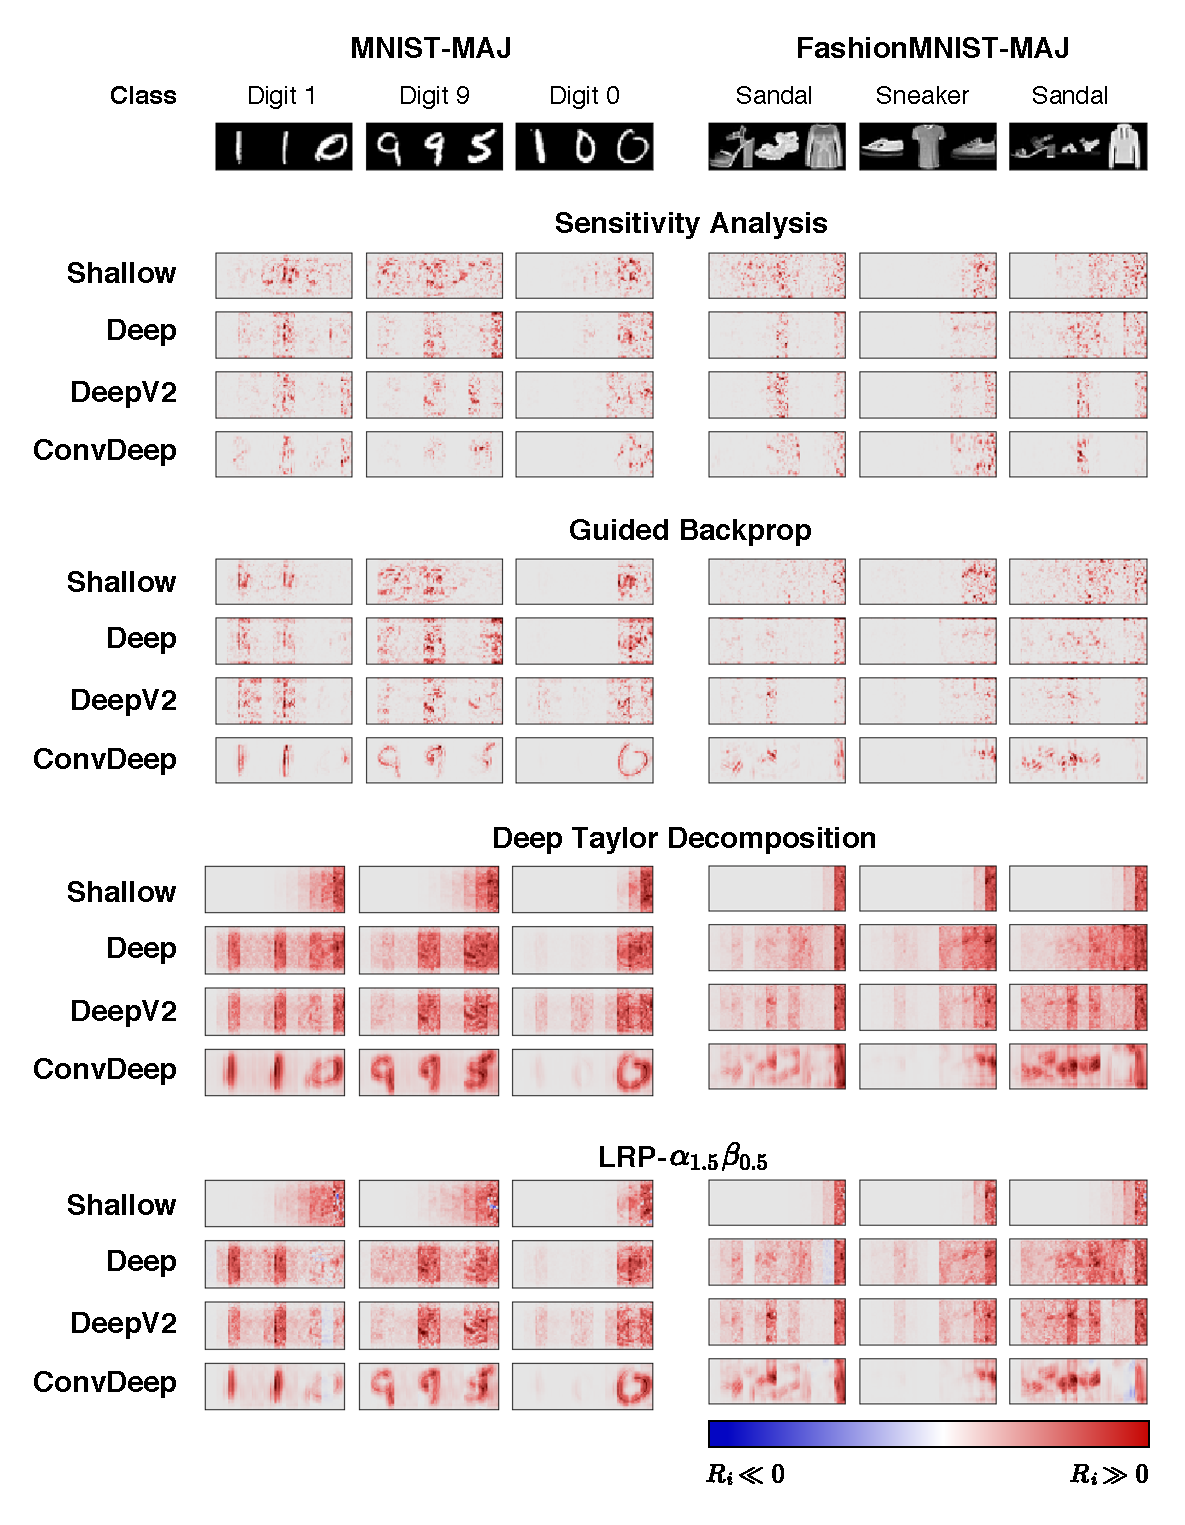
\includegraphics[width=\textwidth]{sketch/heatmap_msc_for_thesis}
\caption{Relevance heatmaps for MSC problem} 
\label{fig:heatmap_msc_mix_for_thesis}
\end{figure}

In this experiment, I chose $T=12$, hence $(\x_t \in \mathbb{R}^{28,7})_{t=1}^{12}$. Table \ref{tab:maj_rnn_model_acc} shows number of trainable variables and accuracy of the trained models. These trained models have equivalent number of variables and accuracy, hence comparing heatmaps of these models is a fair evaluation.

As can be seen from \addfigure{\ref{fig:heatmap_msc_mix_for_thesis}}, the deeper architecture, the fewer relevant scores distributed to irrelevant region. This effect happens across all explanation methods. This result further supports what has shown in Experiment 1.  Moreover, although relevance heatmaps from \rnncellseq{Shallow}{12}, \rnncellseq{Deep}{12}, and \rnncellseq{DeepV2}{12} generally look noisy, increasing the depth of architecture seems to reduce the noise in the heatmaps.   On the other hand, \rnncellseq{ConvDeep}{12} does not  only properly assign relevance quantities to the right time steps, but its heatmaps are also sound. In particular, one can easily perceive features of $\x$ from \rnncellseq{ConvDeep}{12}'s GB and DTD heatmaps.


 \begin{figure}[h]
\centering
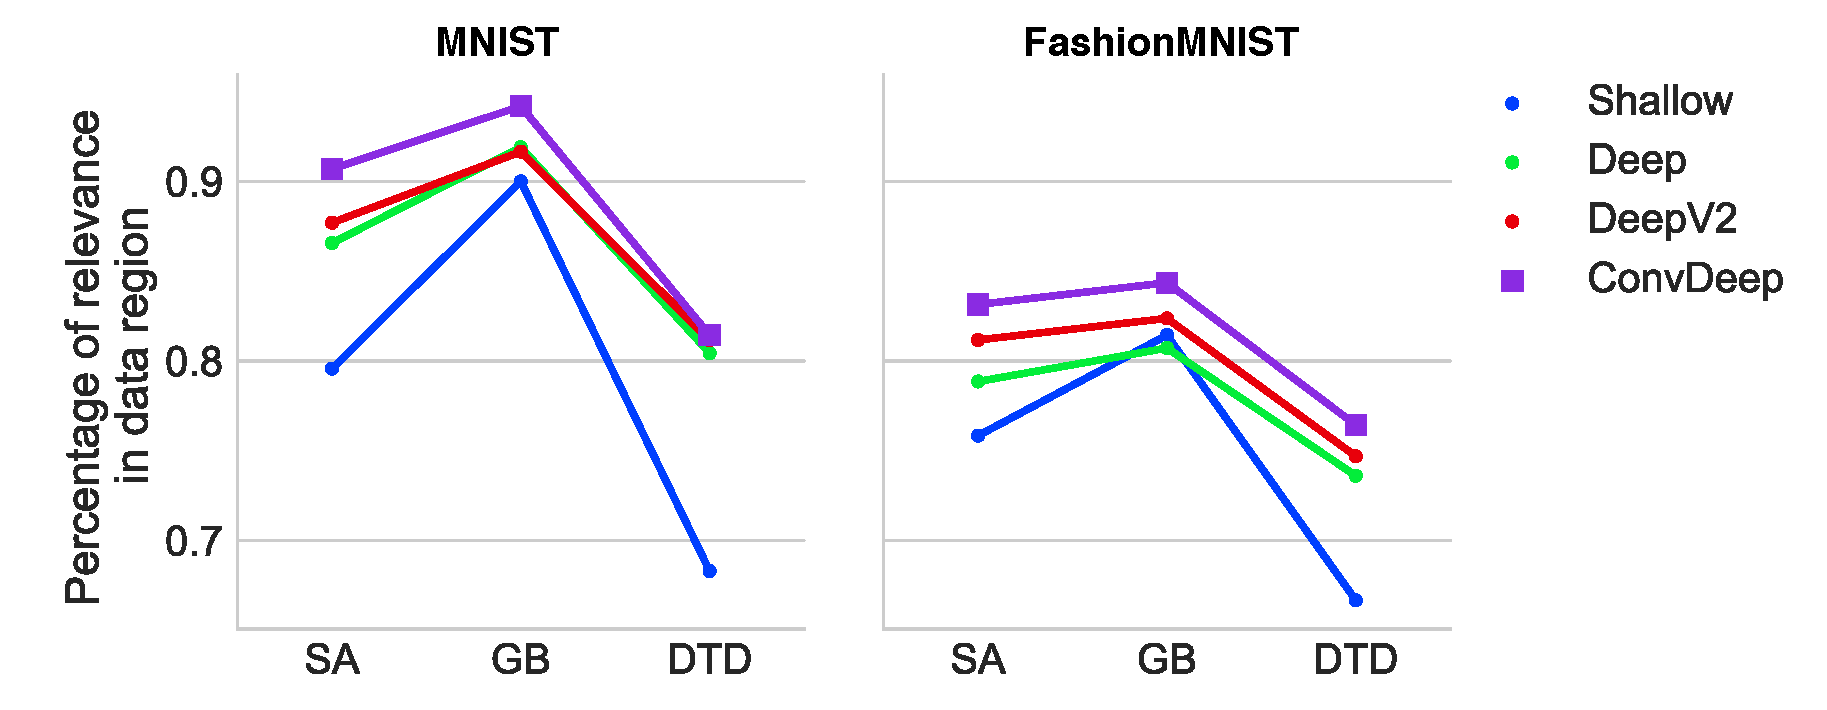
\includegraphics[width=0.7\textwidth]{sketch/rel_dist_maj_3_samples_thesis}
\caption{Percentage of relevance in data region} 
\label{fig:rel_dist_maj_3_samples_thesis}
%todo figure remove lines
\end{figure}

\addfigure{\ref{fig:rel_dist_maj_3_samples_thesis}} presents a quantitive  evaluation of the impact from the depth of architecture to the explanation. Here, the measurement is the percentage of relevance quantities assigned to regions of majority class : these regions are indicated by the red triangles in \addfigure{\ref{fig:heatmap_msc_mix_for_thesis}}, averaged over test sample population. Results from \addfigure{\ref{fig:rel_dist_maj_3_samples_thesis}} indicate that the depth of architecture indeed improves quality of the explanations. In particular, the percentage of correct relevance assignment of each explanation technique increases as more layers introduced. This enhancement can be seen clearly from the result of FashionMNIST. Moreover, as expected, \rnncellseq{ConvDeep}{12} improves the percentage even more. Additionally, we can observe that the difference between the  percentage of the baseline, \rnncellseq{Shallow}{12}, and the deep architectures changes with different proposition across methods. In particular, we see the difference of SA and DTD are slightly larger than the difference of GB. This implies that some explanation methods get more benefit from the depth of architecture.

\todo{add cases that convdeep fail}

\subsection{Summary}
The outcome of this experiment quantitively confirms that the depth of architecture has impacts on explanation of the model. It also shows that  the depth of architecture affects explanation in different level on different methods. More precisely, comparing to guided backprop(GB), quality of sensitivity analysis(SA) and deep Taylor decomposition(DTD) explanation is more depend on the depth.

\section{Experiment 3 : Improve Relevance Propagation}
The results from the previous experiment show that better structured cell architecture leads to better explanation, in other words, easier to be explained. However, there are some cases that the purposed architectures fail to distribute relevance properly.  Hence, this experiment aims to extend the proposed architectures further to better address the problem. More precisely, we consider the same setting as Section \ref{sec:exp2_prob_formulate}. Here, we propose 3 improvements, namely stationary dropout, employing gating units,  and literal connections of convolutional layers.


\subsection{Proposal 1 :  Stationary Dropout}
Dropout is a simple regularization technique that randomly suspends activity of neurons during training\cite{SrivastavaDropoutSimpleWay2014} . This randomized suspension allows the neurons to learn more specific representations and reduces chance of overfitting.  As a result, its influence directly impacts the quality of explanation. 

%\addfigure{\ref{fig:lenet_various_dropout}} shows explanations of LeNet trained with different dropout probability.

%\begin{figure}[!htb]
%\centering
%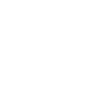
\includegraphics[draft,width=0.5\textwidth]{/sketch/placeholder}
%\caption{LeNet with various dropout values} 
%\label{fig:lenet_various_dropout}  
%\end{figure}



\begin{figure}[!htb]
\centering
\subfloat[Naive Dropout]{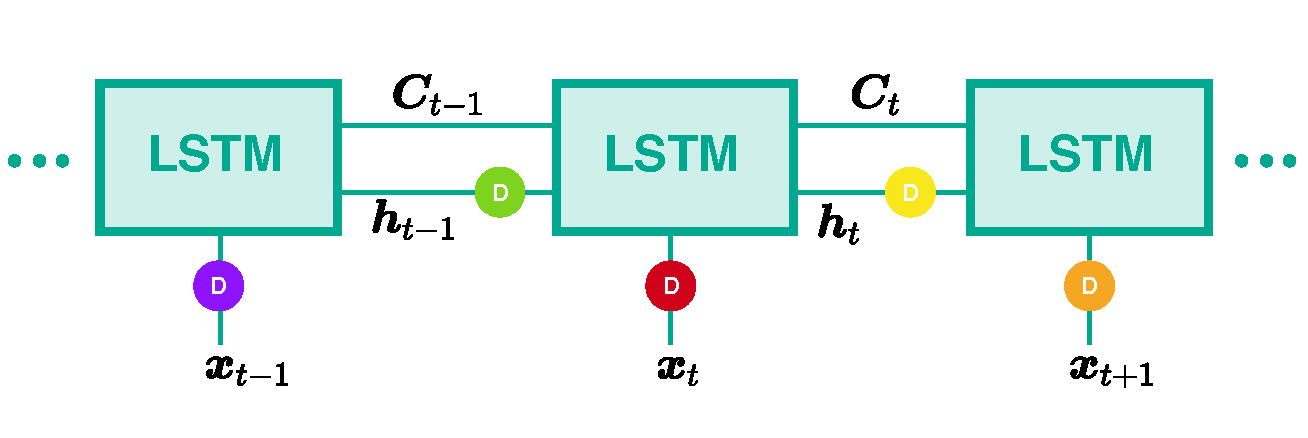
\includegraphics[width=0.8\textwidth]{sketch/lstm_naive_dropout} \label{fig:lstm_naive_dropout}} \\
\subfloat[Stationary Dropout]{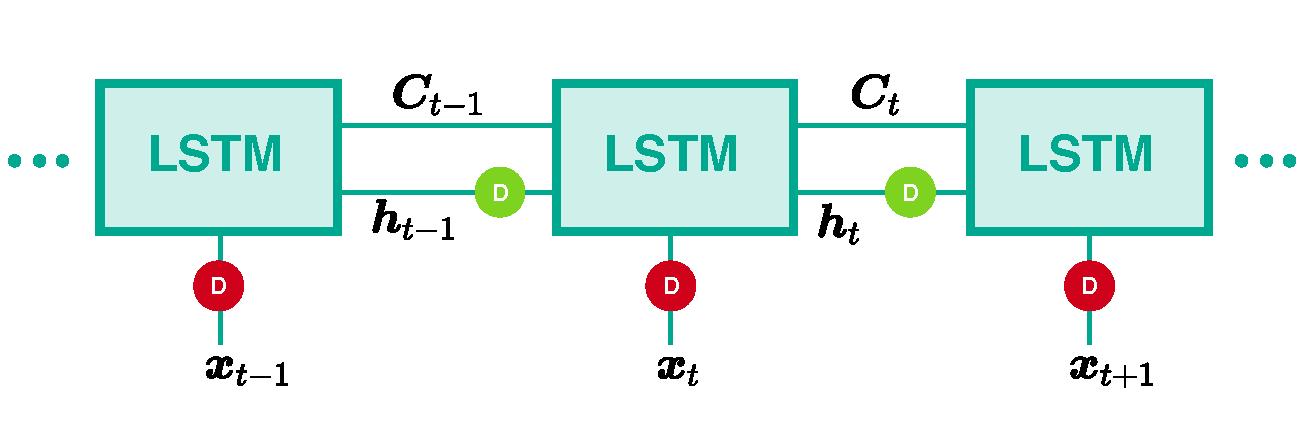
\includegraphics[width=0.8\textwidth]{sketch/lstm_variational_dropout} \label{fig:lstm_variational_dropout}}

\patcaption{LSTM with different dropout approaches.}{\textcircled{\tiny \textbf D} indicates a dropout mask and its color represents the suspension activity.}
\label{fig:dropout_lstm}
\end{figure}

However, unlike typical feedforward architectures, RNN layers are reused across time step, hence a question arises whether the same neurons in those layers should be suspended or they should be different neurons when applying the layers multiple times. \addfigure{\ref{fig:dropout_lstm}} illustrates these 2 different approaches where different colors represent different dropping activities. In particular, this stationary dropout was first proposed by \cite{GalTheoreticallyGroundedApplication2016} who applied  the technique to LSTM and GRU and found accuracy improvements on language modeling tasks.

\subsection{Proposal 2 : Gating units}
\begin{figure}[!htb]
\centering
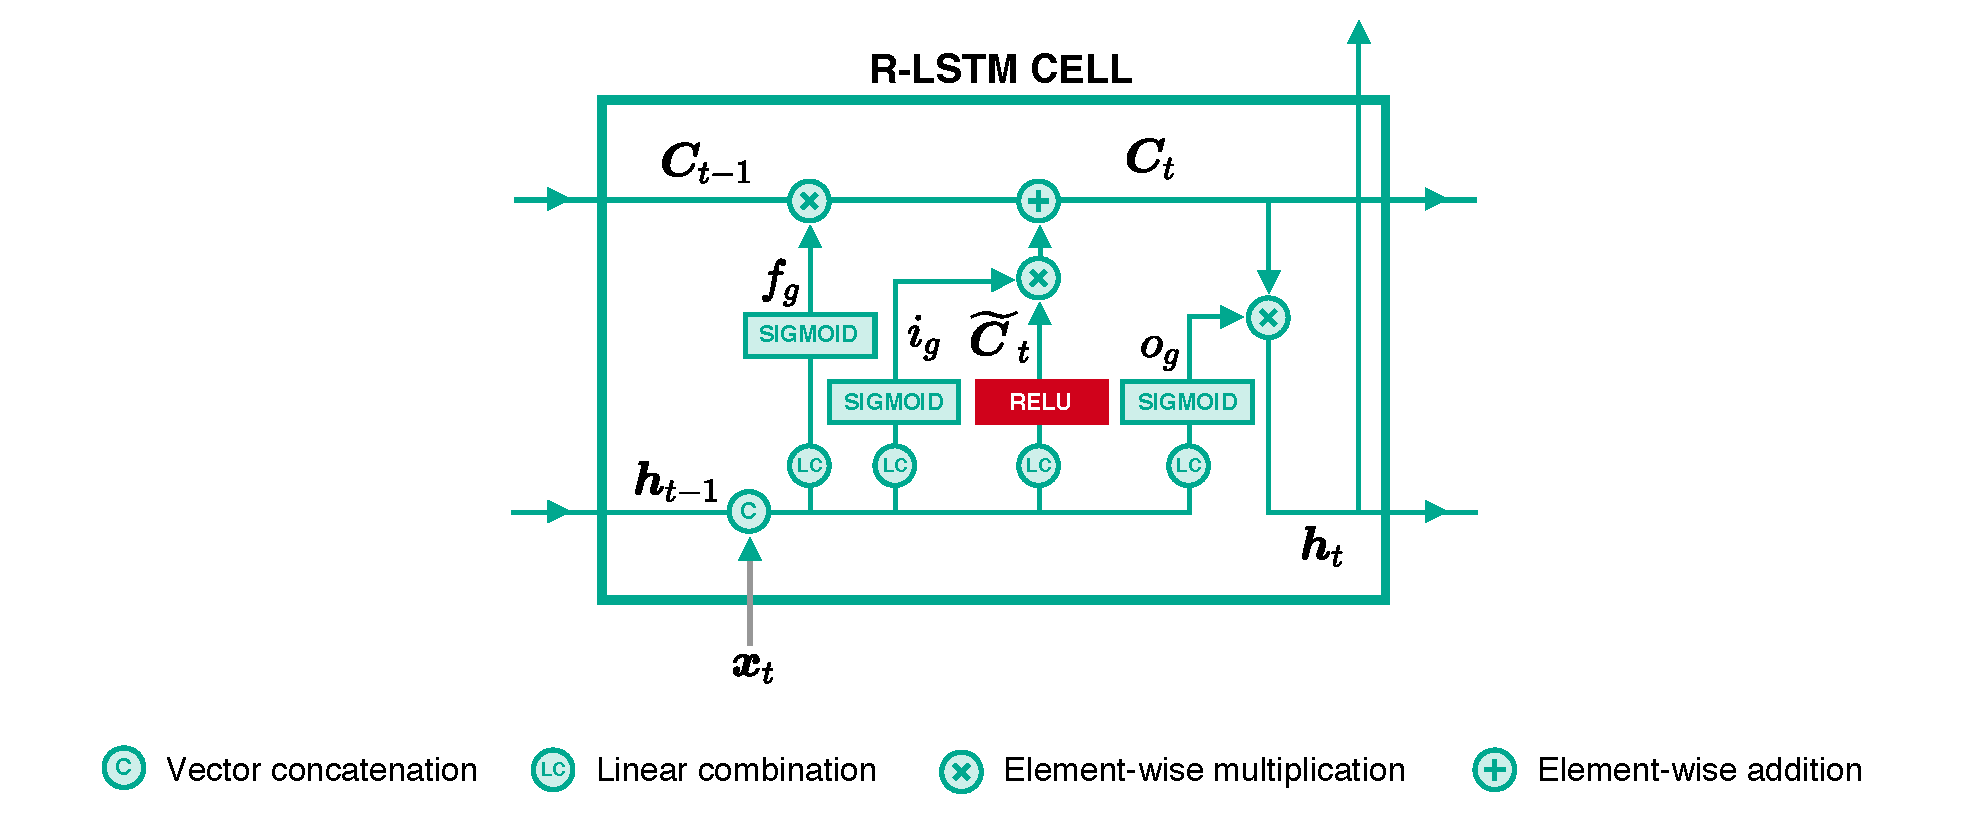
\includegraphics[width=1\textwidth]{sketch/relu_lstm}
\caption{R-LSTM Structure} 

\label{fig:relu_lstm} 
\end{figure}

It is already shown that gating units and addictive updates are critical mechanisms that enable LSTM to learn long term dependencies \cite{GreffLSTMsearchspace2017, Jozefowiczempiricalexplorationrecurrent2015a}. However, LSTM is not readily applicable for methods we are considering in this thesis. More precisely, the use of sigmoid and tanh activations violates the assumption of GB and DTD. Therefore, we propose a slight modified version of LSTM where ReLU activations are used to compute cell state candidates $\widetilde{C}_t$ instead of tanh functions. This results $C_t \in \mathbb{R}^+$, hence the tanh activation for $h_t$  is also removed.  Sigmoid activations are treated as constants when applying DTD and LRP, while its gradients are set to zero for GB. We refer this architecture as R-LSTM to differentiate from the original.  \addfigure{\ref{fig:relu_lstm}} presents an overview of R-LSTM architecture.


\subsection{Proposal 3 : Convolutional layer with literal connections}
As discussed in Section \ref{sec:conv}, convolution and pooling operator enable neural networks to learn hierarchical and invariant representations, which are directly beneficial to explanation quality. Because the \rnncell{ConvDeep} architecture we proposed in Section \ref{sec:exp2} does not seem to exploit this properly because it has recurrent connections only layers after the convolutional and pooling layers. This can be analogically viewed that the ConvDeep architecture only shares high-level features between step instead of low-level features. This might lead to obscure low-level features in the explanation. 

%In this proposal, we aims to share those low-level features to convolutional operators of the next step as well. We call this connections as \textit{literal connections} and   We are going to refer Conv$^+$ to the setting that employs convolutional layers with literal connections.


 \begin{figure}[!htb]
\centering
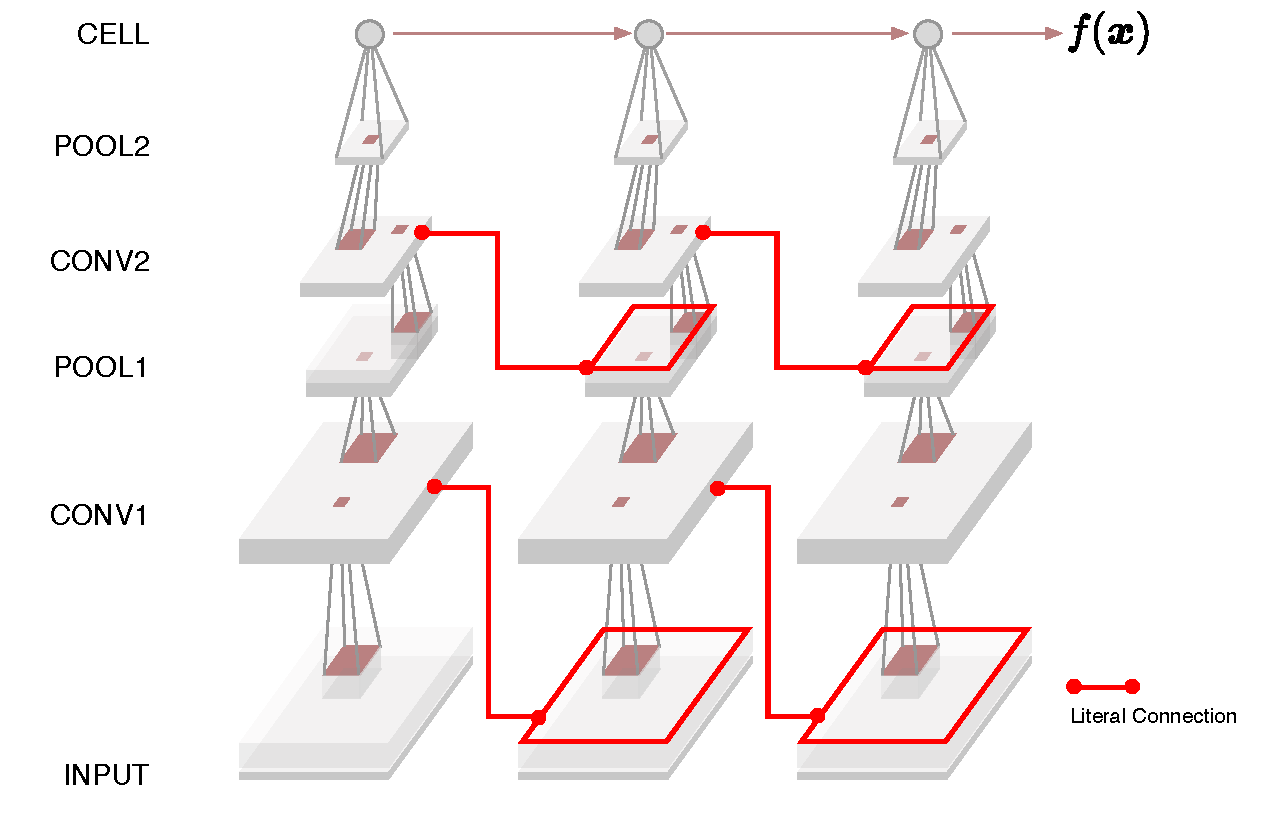
\includegraphics[width=\textwidth]{sketch/conv_literalconn}
\patcaption{ConvDeep with literal connections}{(\rnncell{Conv$^+$Deep}).} 
\label{fig:conv_literalconn}
\end{figure}

Therefore, we propose to also share results from convolution operators to the operators in the next step. We name this connections as \textit{literal connections} and \addfigure{\ref{fig:conv_literalconn}} illustrates such connections in red. From the following, we are going to refer Conv$^+$ to the setting where convolutional layers are connected through the literal connections. 

%\subsection{Setting}
In this experiment, we divided results into 2 parts. The first part focuses on stationary dropout and R-LSTM proposal and use the Deep architecture as a baseline. We refer models trained with stationary dropout with $-SD$ suffix. For R-LSTM's configuration, we also added one layer with 256 neurons between the input and 75 R-LSTM cells to make it comparable to the Deep architecture.  \todo{Figure X : show R-LSTM setting}

In the second part, we are going to discuss results from the literal connection proposal as well as results from ConvR-LSTM where the first fully-connected layer is replaced by convolutions and pooling layers with the same configuration as in ConvDeep. The number of R-LSTM cells is also the same to the first part. 

\todo{figure describe R-LSTM settings with cell?}


\subsection{Result}
Table \ref{tab:maj_exp3_model_acc} shows number of trainable parameters in the proposed architectures as well as accuracy.

\renewcommand{\arraystretch}{1.5}
\begin{table}[h]
\begin{center}
\begin{tabular}{lc|c|c|}
\cline{3-4}
& &
\multicolumn{2}{c|}{\parbox{3.5cm}{ \vskip 1mm \centering \textbf{Accuracy} \vskip 1mm}} \\ \hline
\multicolumn{1}{|l|}{\textbf{Cell architecture}} & \textbf{No. variables} & \textbf{MNIST-MAJ} & \textbf{FashionMNIST-MAJ} \\ \hline
\multicolumn{1}{|l|}{Deep-SD}                  & 153,578             & 98.10\% & 89.47\% \\ 
\multicolumn{1}{|l|}{R-LSTM}                    & 145,701   & 98.50\% & 91.35\% \\ 
\multicolumn{1}{|l|}{R-LSTM-SD}              &  145,701                & 98.57\% & 91.52\% \\ 
 \multicolumn{1}{|l|}{Conv$^+$Deep}       & 175,418                 & 97.92\% & 88.10\% \\
 \multicolumn{1}{|l|}{ConvR-LSTM-SD}      & 152,125                 & 99.35\% & 93.60\%  \\ 
\multicolumn{1}{|l|}{Conv$^+$R-LSTM-SD}   & 175,741                & 98.48\% & 88.19	\%  \\ \hline 
\end{tabular}

\end{center}
\caption{Number of trainable variables and model accuracy of the  proposed architectures for MNIST-MAJ and FashionMNIST-MAJ.}
\label{tab:maj_exp3_model_acc}
\end{table}
\renewcommand{\arraystretch}{1}


\subsubsection{Stationary Dropout and R-LSTM}
 \begin{figure}[!htb]
\centering
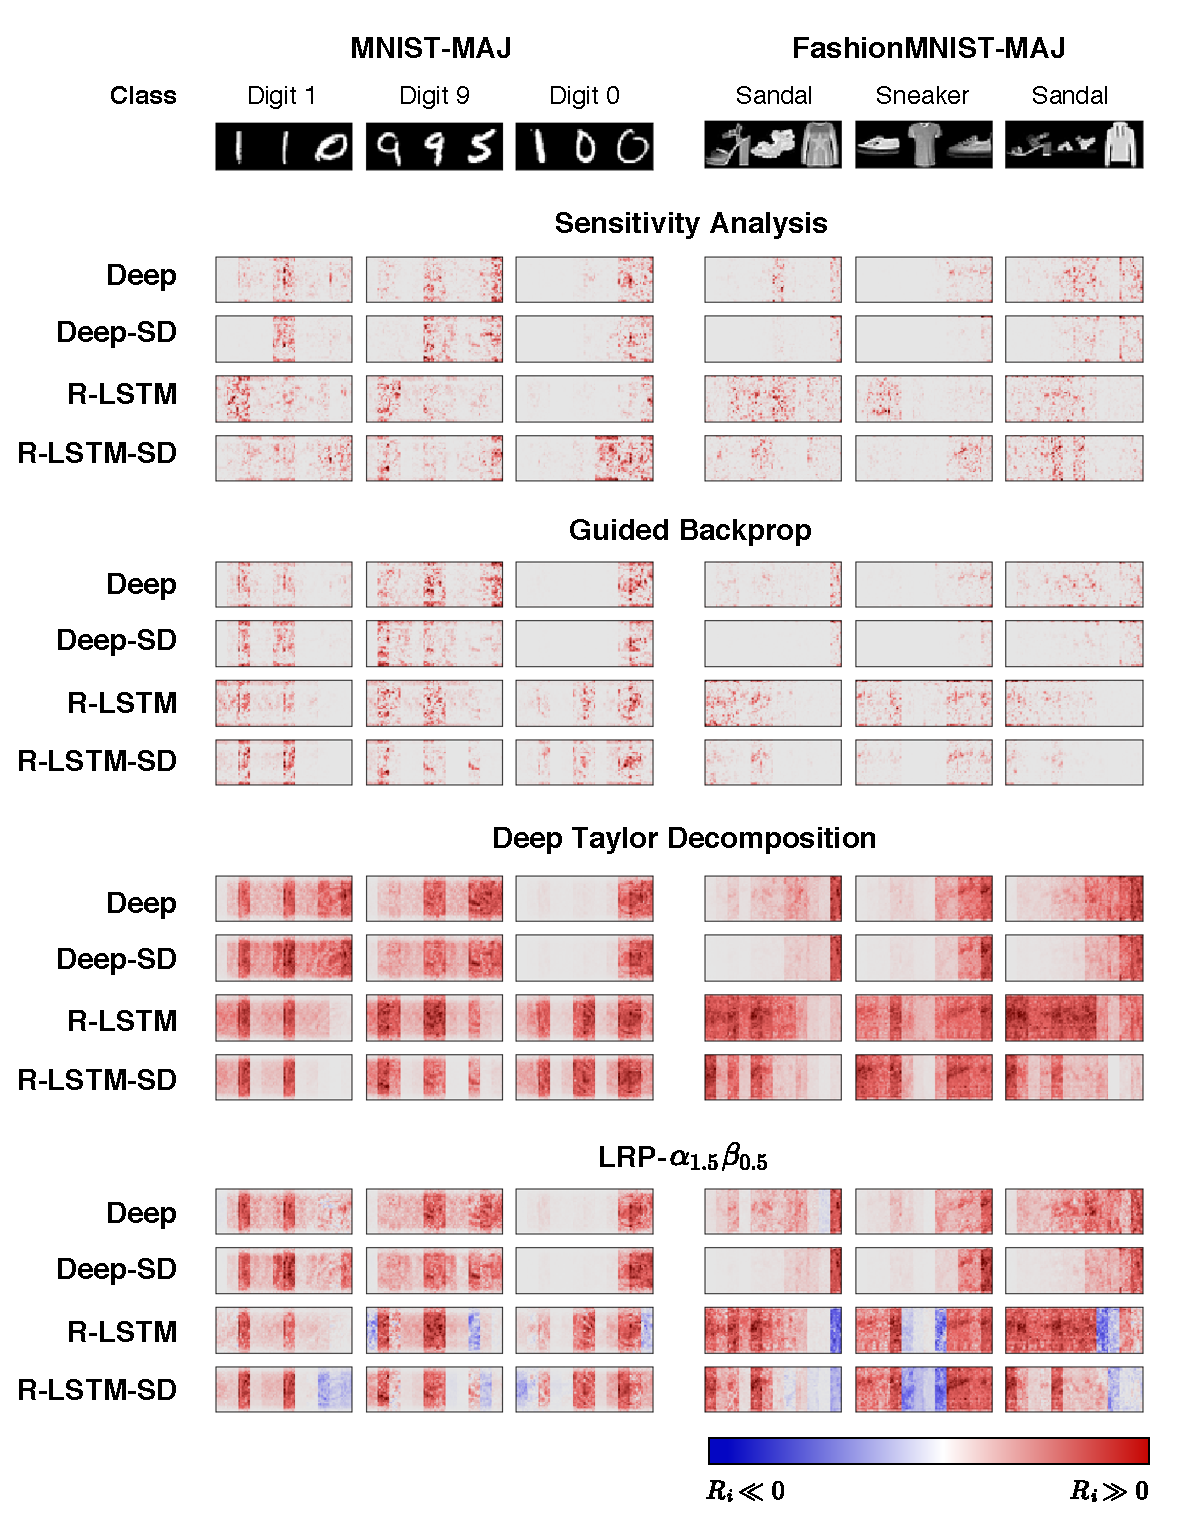
\includegraphics[width=\textwidth]{sketch/heatmap_msc_rlstm_exp}
\patcaption{Relevance heatmaps produced by different explanation techniques on Deep and R-LSTM architecture trained on MNIST-MAJ and FashionMNIST-MAJ with sequence length $T=12$ and different dropout configurations.}{\heatmapscaleexplain} 
\label{fig:heatmap_msc_rlstm_exp}
\end{figure}

\addfigure{\ref{fig:heatmap_msc_rlstm_exp}} shows results of the first part of this experiment. Here, variants of Deep and R-LSTM are compared. From the figure, it is obvious that R-LSTM provides better explanations than the Deep architecture. More precisely, we can directly observe the improvements from GB, DTD and $\lrpp$ heatmaps. Moreover, training with stationary dropout seems to produce R-LSTM with higher explanation capability. This is well notable on explanations from  DTD and $\lrpp$. In contrast, stationary dropout does not seem to have any prominent impact on the Deep architecture.


 \begin{figure}[!htb]
\centering
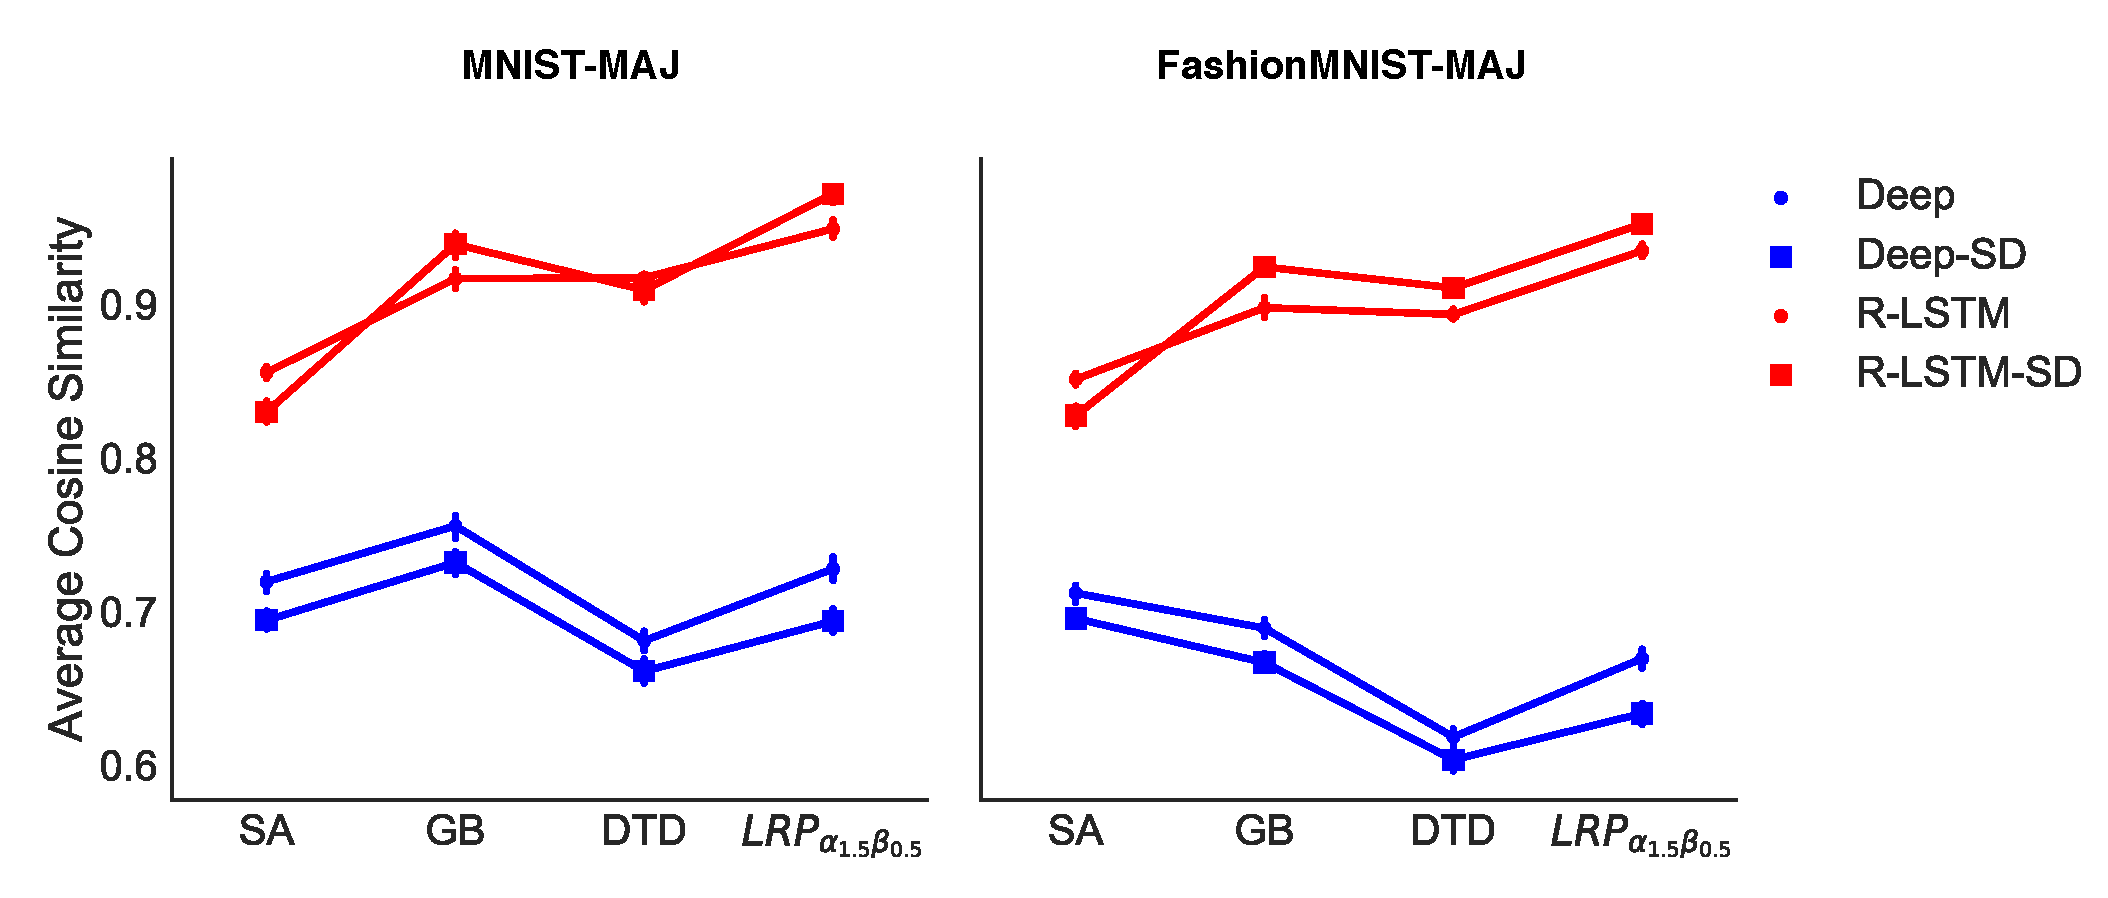
\includegraphics[width=\textwidth]{sketch/rel_dist_rlstm_exp}
%\caption{}  }. 
\patcaption{Average cosine similarity from different explanation techniques and Deep and R-LSTM architecture.}{The values are averaged from cross-validation results and the vertical lines depicted 95\% confidence interval. The baseline is the Deep architecture depicted by dotted blue line. Accuracy of the models can be found at Appendix  \ref{annex:model_acc}}

\label{fig:rel_dist_rlstm_exp}
\end{figure}

\addfigure{\ref{fig:rel_dist_rlstm_exp}} presents the quantitative evaluation. As a reminder, these plots are cosine similarity averaged over models trained with cross validation procedure described in  Section \ref{sec:evaluation_med}. The figure shows that R-LSTM significantly improves relevance distribution than the Deep architecture regardless of explanation techniques.  This means that R-LSTM is more explainable than the Deep architecture. Similar to one observation in Section \ref{sec:exp1_result}, we also see that the proportion of the improvement of DTD and LRP seem to have greater advantage from R-LSTM than the other methods.  

\addfigure{\ref{fig:rel_dist_rlstm_exp}}  also shows another interesting result. We can see that R-LSTM trained with stationary dropout, or R-LSTM-SD, produces better explanations than R-LSTM on FashionMNIST-MAJ, although the difference does not obvious on MNIST-MAJ. This might be due to complexity of FashionMNIST samples' structures, as a result keeping dropout mask the same for all step would enable the network to efficiently learn latent features from homogenous input. In contrast, this does not seem to be the case for the Deep architecture. Particularly, we find that the cosine similarity measurement of Deep-SD is lower than Deep in any case.

\todo{hypo thesis?}
\clearpage

\subsubsection{ConvDeep with literal connections and ConvR-LSTM}
 \begin{figure}[!htb]
\centering
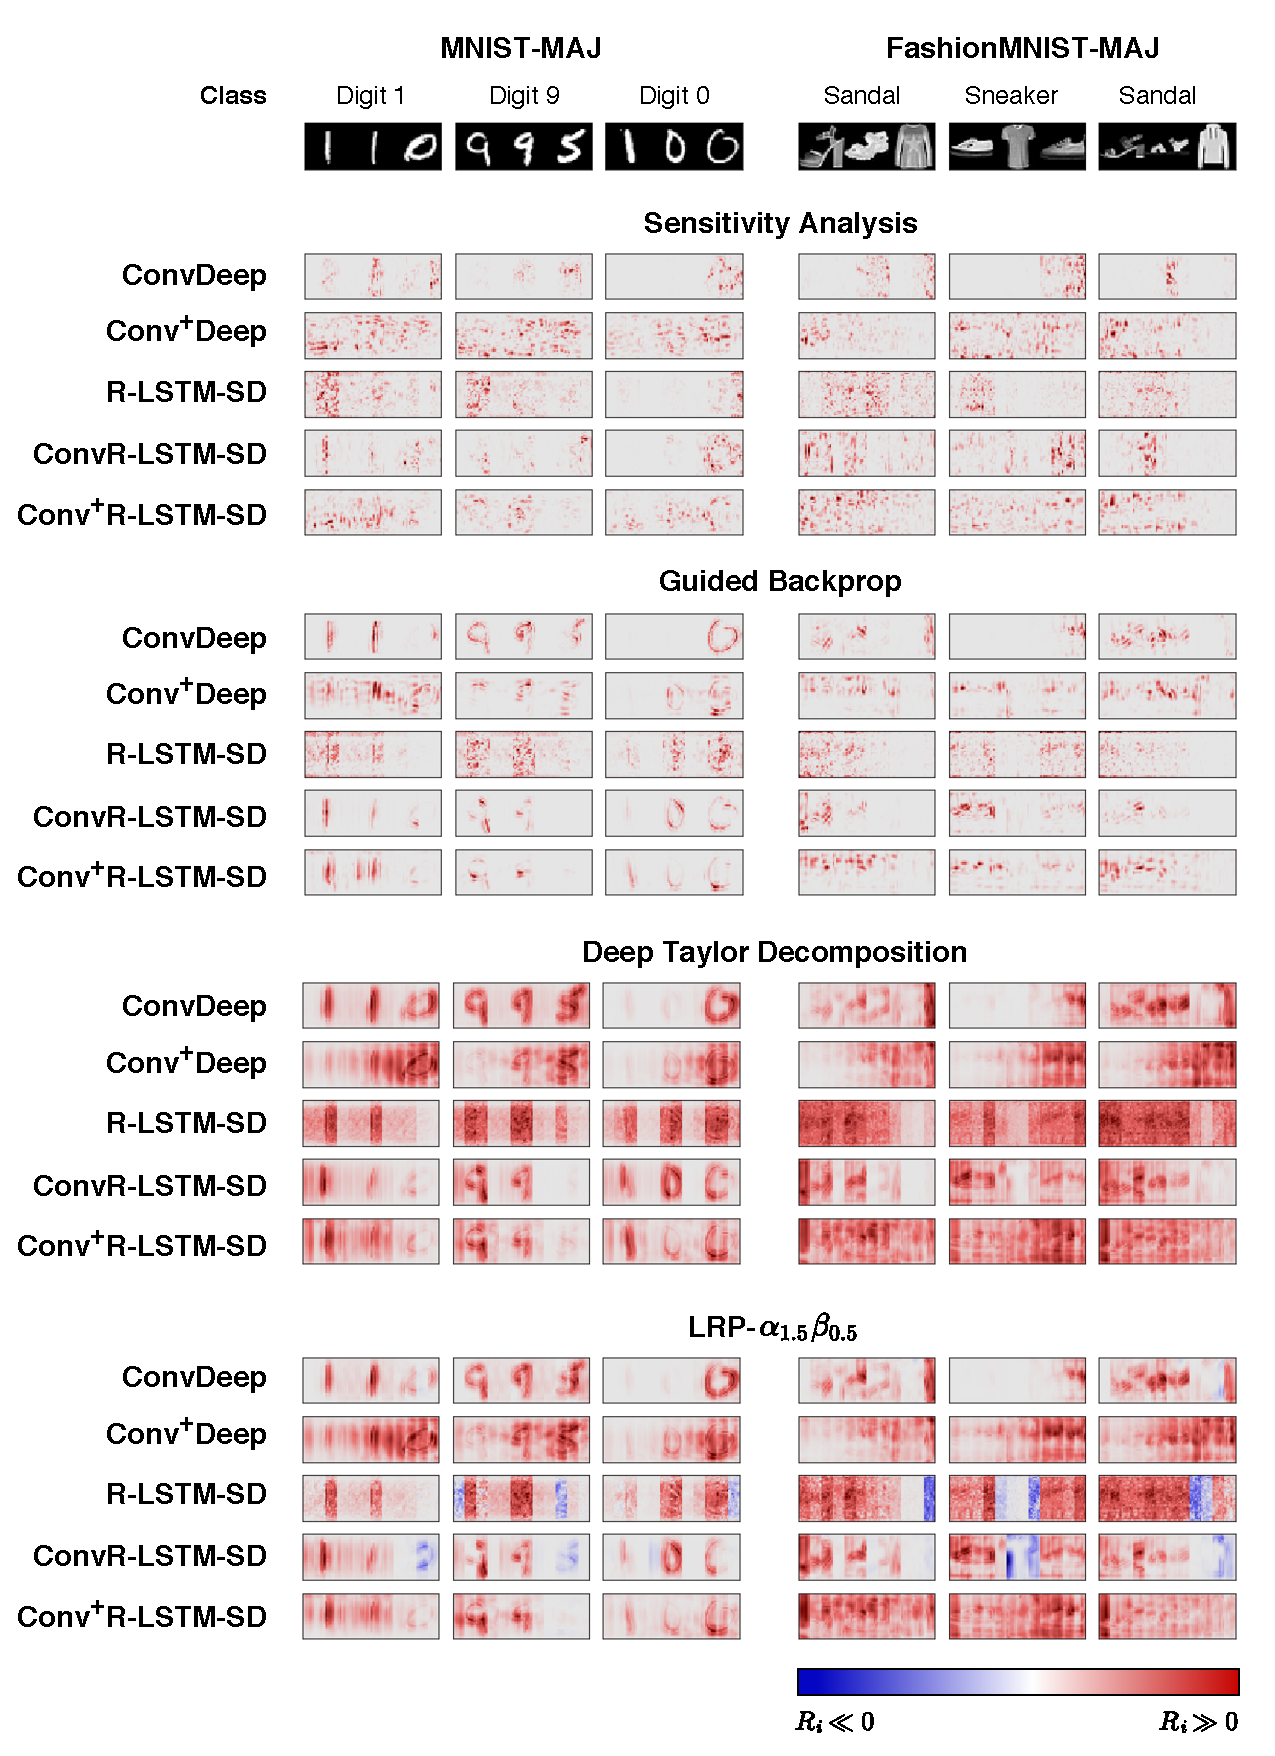
\includegraphics[width=\textwidth]{sketch/heatmap_msc_convtran_exp_v2}
\patcaption{Relevance heatmaps produced by different explanation techniques on variants of ConvDeep and R-LSTM architecture trained on MNIST-MAJ and FashionMNIST-MAJ with sequence length $T=12$.}{\heatmapscaleexplain} 
\label{fig:heatmap_msc_convtran_exp}
\end{figure}
For the second part, we compare the ConvDeep architecture and the effect of literal connections as well as R-LSTM-SD with convolutional layers, which is referred as ConvR-LSTM-SD. According to \addfigure{\ref{fig:heatmap_msc_convtran_exp}}, Conv$^+$Deep produces more diffuse relevance heatmaps than ConvDeep. This is specially notable on heatmaps from SA  and GB method. Similarly, Conv$^+$Deep also produces worse results for DTD and $\lrpp$, for example consider Digit 1 and Digit 9 sample, where the relevance scores are unnecessarily distributed to the last digit's block. 

\addfigure{\ref{fig:heatmap_msc_convtran_exp}} also shows relevance heatmaps from ConvR-LSTM-SD whose first fully-connected layer is replaced by 2 convolutional and pooling layers. Comparing to R-LSTM-SD, having convolutional and pooling layers does improve  the quality of the heatmaps further. In particular, we can clearly see samples' structures from the explanations. \addfigure{\ref{fig:heatmap_msc_convrlstm_pos_rel}} further emphasizes the improvement introduced by the convolutional and pooling layers. Here, we plots the relevance heatmaps by using only positive relevance. We can see that the heatmaps from ConvR-LSTM-SD are proper highlighted and provide substantial  features of the samples.

 \begin{figure}[!htb]
\centering
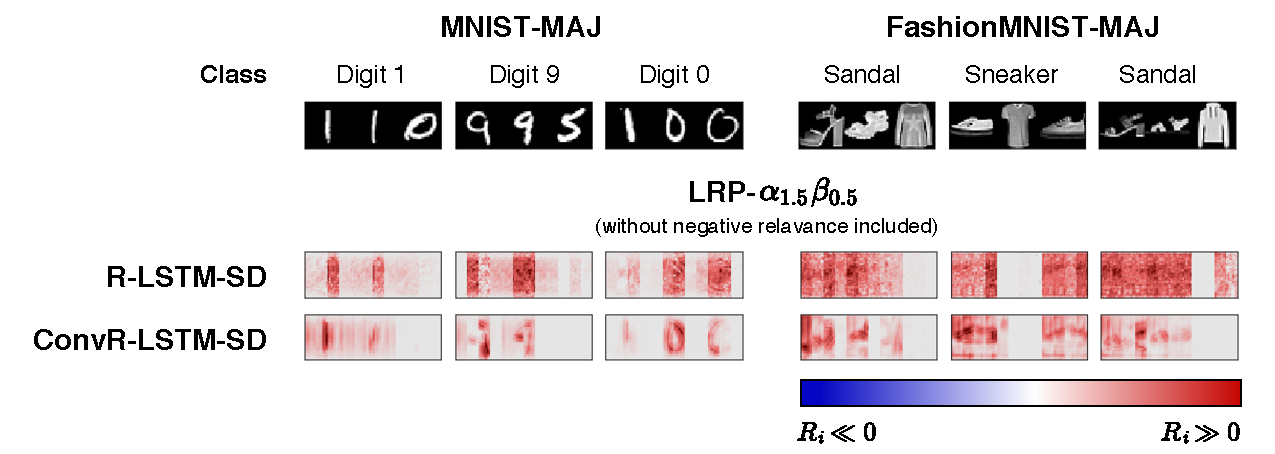
\includegraphics[width=\textwidth]{sketch/heatmap_msc_convrlstm_pos_rel}
\patcaption{Positive relevance heatmaps produced by $\lrpp$ technique on R-LSTM and ConvR-LSTM architecture trained on MNIST-MAJ and FashionMNIST-MAJ with sequence length $T=12$.}{\heatmapscaleexplain} 
\label{fig:heatmap_msc_convrlstm_pos_rel}
\end{figure}

 \begin{figure}[!htb]
\centering
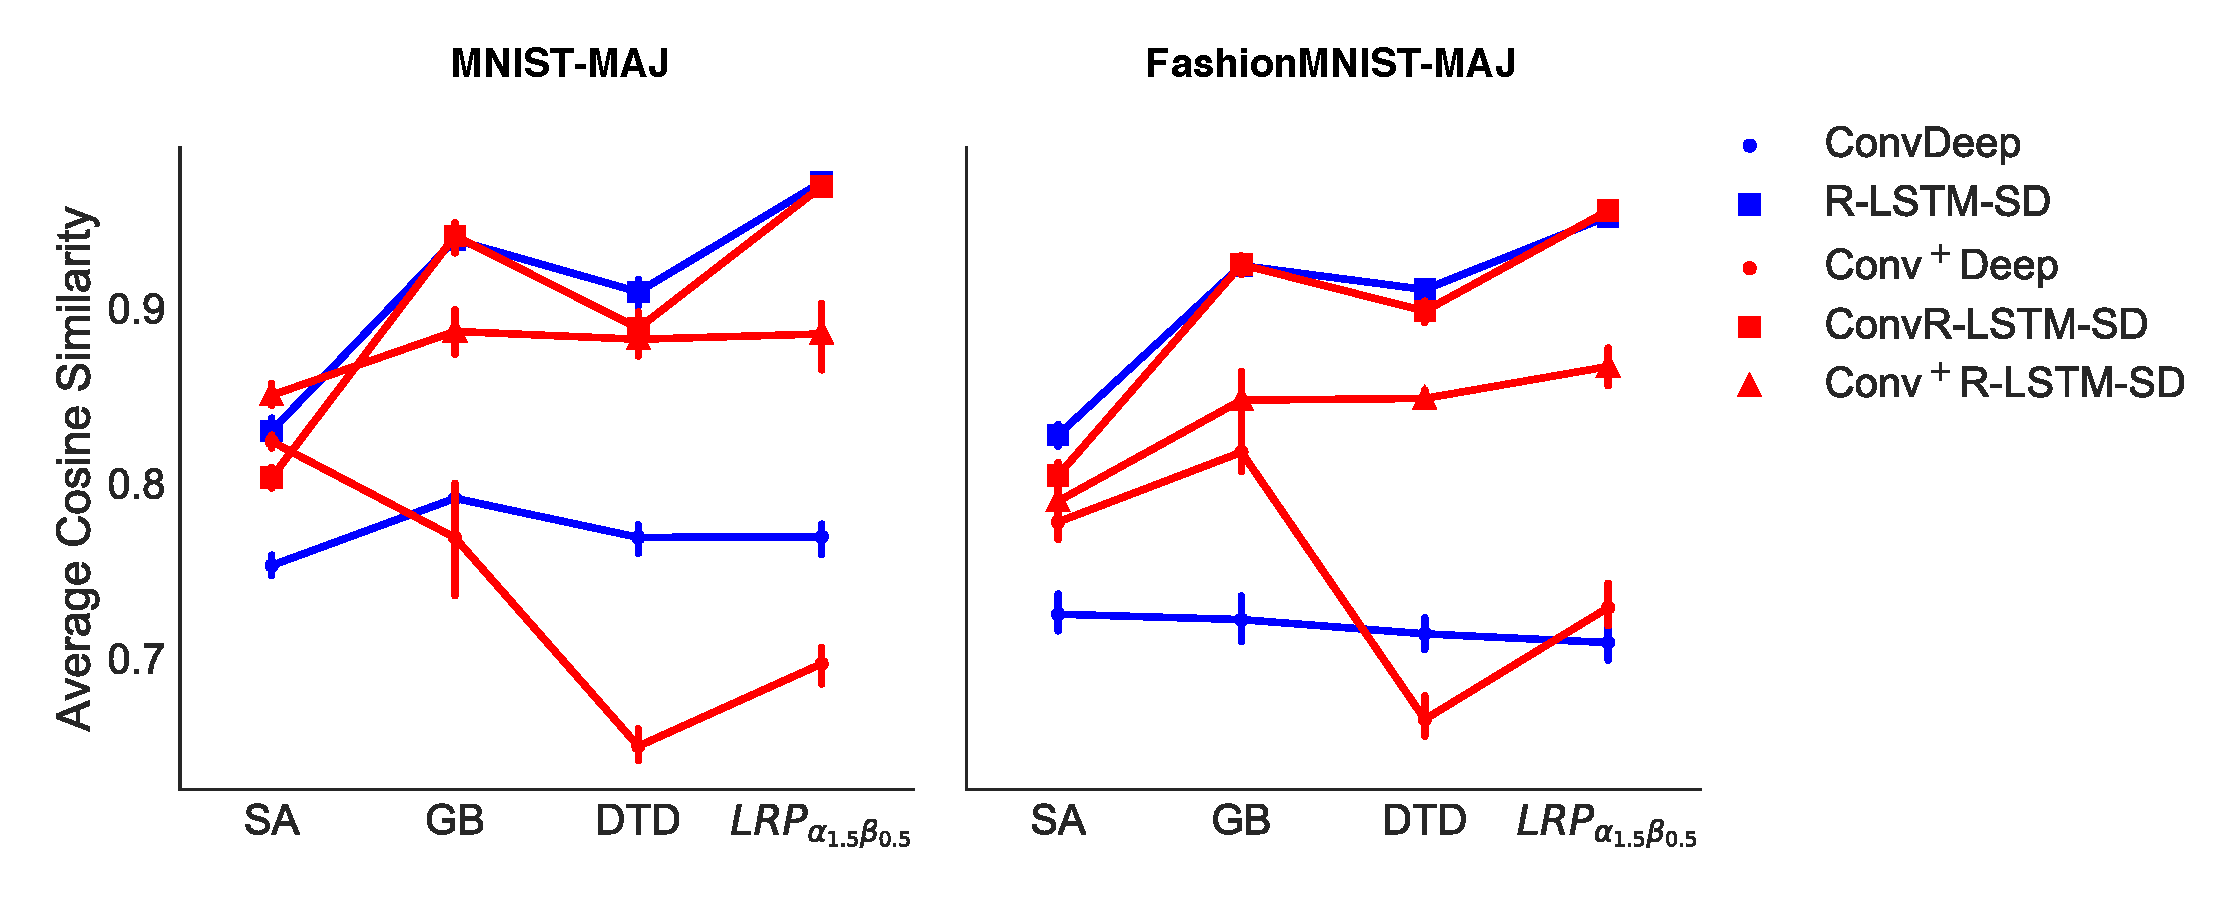
\includegraphics[width=\textwidth]{sketch/rel_dist_convdeep_trans_exp}
\patcaption{Average cosine similarity from different explanation techniques and variants of ConvDeep and R-LSTM architecture.}{The values are averaged from cross-validation results and the vertical lines depicted 95\% confidence interval. The baseline are the Deep and R-LSTM-SD architecture represented in blue. Accuracy of the models can be found at Appendix \ref{annex:model_acc}} 
\label{fig:rel_dist_convdeep_trans_exp}
\end{figure}

\addfigure{\ref{fig:rel_dist_convdeep_trans_exp}} presents the cosine similarity measurement this second part of the experiment. Here, ConvDeep and R-LSTM-SD are results from the previous experiments and used as baseline. Unexpectedly, having literal connections in ConvDeep does not seem to show consistent influence between MNIST-MAJ and FashionMNIST-MAJ. However, the connections considerably reduce the explanation capability of the ConvR-LSTM-SD architecture. 
 Although explanations from ConvR-LSTM-SD are less noisy and contain impressive structures from the input as shown in \addfigure{\ref{fig:heatmap_msc_convrlstm_pos_rel}}, the average cosine similarity of R-LSTM-SD and ConvR-LSTM-SD look almost identical. This is due to the fact our cosine similarity measurement operates on scalar values but not structures inside explanation heatmaps.
 
 \todo{hypo: In fact, using Tukey HSD test shows that the improvement is not statistically significant} 
\todo{hypothesis testing}

\clearpage

\subsection{Summary}
Results from this experiment shows some successful improvements from what we have seen on Sectoin \ref{sec:exp2}. In particular, employing gating unit and keeping dropout activities the same significantly improve explanation ability of RNN models on any explanation method.  

Moreover, convolutional and pooling layers enables the models to produce explanations with more perceivable input features than traditional fully-connected layers, although this improvement does not seem to be well captured by cosine similarity that we proposed to use. . This illustrates  a shortcoming of cosine similarity that we proposed to use for the quantitative evaluation.

On the other hand, literal connections do not show any consistent improvement for the settings we are considering. In fact, having wider confidence interval suggests that they seem to make explanations less stable.

